\documentclass[11pt]{article}

    \usepackage[breakable]{tcolorbox}
    \usepackage{parskip} % Stop auto-indenting (to mimic markdown behaviour)
    
    \usepackage{iftex}
    \ifPDFTeX
    	\usepackage[T1]{fontenc}
    	\usepackage{mathpazo}
    \else
    	\usepackage{fontspec}
    \fi

    % Basic figure setup, for now with no caption control since it's done
    % automatically by Pandoc (which extracts ![](path) syntax from Markdown).
    \usepackage{graphicx}
    % Maintain compatibility with old templates. Remove in nbconvert 6.0
    \let\Oldincludegraphics\includegraphics
    % Ensure that by default, figures have no caption (until we provide a
    % proper Figure object with a Caption API and a way to capture that
    % in the conversion process - todo).
    \usepackage{caption}
    \DeclareCaptionFormat{nocaption}{}
    \captionsetup{format=nocaption,aboveskip=0pt,belowskip=0pt}

    \usepackage{float}
    \floatplacement{figure}{H} % forces figures to be placed at the correct location
    \usepackage{xcolor} % Allow colors to be defined
    \usepackage{enumerate} % Needed for markdown enumerations to work
    \usepackage{geometry} % Used to adjust the document margins
    \usepackage{amsmath} % Equations
    \usepackage{amssymb} % Equations
    \usepackage{textcomp} % defines textquotesingle
    % Hack from http://tex.stackexchange.com/a/47451/13684:
    \AtBeginDocument{%
        \def\PYZsq{\textquotesingle}% Upright quotes in Pygmentized code
    }
    \usepackage{upquote} % Upright quotes for verbatim code
    \usepackage{eurosym} % defines \euro
    \usepackage[mathletters]{ucs} % Extended unicode (utf-8) support
    \usepackage{fancyvrb} % verbatim replacement that allows latex
    \usepackage{grffile} % extends the file name processing of package graphics 
                         % to support a larger range
    \makeatletter % fix for old versions of grffile with XeLaTeX
    \@ifpackagelater{grffile}{2019/11/01}
    {
      % Do nothing on new versions
    }
    {
      \def\Gread@@xetex#1{%
        \IfFileExists{"\Gin@base".bb}%
        {\Gread@eps{\Gin@base.bb}}%
        {\Gread@@xetex@aux#1}%
      }
    }
    \makeatother
    \usepackage[Export]{adjustbox} % Used to constrain images to a maximum size
    \adjustboxset{max size={0.9\linewidth}{0.9\paperheight}}

    % The hyperref package gives us a pdf with properly built
    % internal navigation ('pdf bookmarks' for the table of contents,
    % internal cross-reference links, web links for URLs, etc.)
    \usepackage{hyperref}
    % The default LaTeX title has an obnoxious amount of whitespace. By default,
    % titling removes some of it. It also provides customization options.
    \usepackage{titling}
    \usepackage{longtable} % longtable support required by pandoc >1.10
    \usepackage{booktabs}  % table support for pandoc > 1.12.2
    \usepackage[inline]{enumitem} % IRkernel/repr support (it uses the enumerate* environment)
    \usepackage[normalem]{ulem} % ulem is needed to support strikethroughs (\sout)
                                % normalem makes italics be italics, not underlines
    \usepackage{mathrsfs}
    

    
    % Colors for the hyperref package
    \definecolor{urlcolor}{rgb}{0,.145,.698}
    \definecolor{linkcolor}{rgb}{.71,0.21,0.01}
    \definecolor{citecolor}{rgb}{.12,.54,.11}

    % ANSI colors
    \definecolor{ansi-black}{HTML}{3E424D}
    \definecolor{ansi-black-intense}{HTML}{282C36}
    \definecolor{ansi-red}{HTML}{E75C58}
    \definecolor{ansi-red-intense}{HTML}{B22B31}
    \definecolor{ansi-green}{HTML}{00A250}
    \definecolor{ansi-green-intense}{HTML}{007427}
    \definecolor{ansi-yellow}{HTML}{DDB62B}
    \definecolor{ansi-yellow-intense}{HTML}{B27D12}
    \definecolor{ansi-blue}{HTML}{208FFB}
    \definecolor{ansi-blue-intense}{HTML}{0065CA}
    \definecolor{ansi-magenta}{HTML}{D160C4}
    \definecolor{ansi-magenta-intense}{HTML}{A03196}
    \definecolor{ansi-cyan}{HTML}{60C6C8}
    \definecolor{ansi-cyan-intense}{HTML}{258F8F}
    \definecolor{ansi-white}{HTML}{C5C1B4}
    \definecolor{ansi-white-intense}{HTML}{A1A6B2}
    \definecolor{ansi-default-inverse-fg}{HTML}{FFFFFF}
    \definecolor{ansi-default-inverse-bg}{HTML}{000000}

    % common color for the border for error outputs.
    \definecolor{outerrorbackground}{HTML}{FFDFDF}

    % commands and environments needed by pandoc snippets
    % extracted from the output of `pandoc -s`
    \providecommand{\tightlist}{%
      \setlength{\itemsep}{0pt}\setlength{\parskip}{0pt}}
    \DefineVerbatimEnvironment{Highlighting}{Verbatim}{commandchars=\\\{\}}
    % Add ',fontsize=\small' for more characters per line
    \newenvironment{Shaded}{}{}
    \newcommand{\KeywordTok}[1]{\textcolor[rgb]{0.00,0.44,0.13}{\textbf{{#1}}}}
    \newcommand{\DataTypeTok}[1]{\textcolor[rgb]{0.56,0.13,0.00}{{#1}}}
    \newcommand{\DecValTok}[1]{\textcolor[rgb]{0.25,0.63,0.44}{{#1}}}
    \newcommand{\BaseNTok}[1]{\textcolor[rgb]{0.25,0.63,0.44}{{#1}}}
    \newcommand{\FloatTok}[1]{\textcolor[rgb]{0.25,0.63,0.44}{{#1}}}
    \newcommand{\CharTok}[1]{\textcolor[rgb]{0.25,0.44,0.63}{{#1}}}
    \newcommand{\StringTok}[1]{\textcolor[rgb]{0.25,0.44,0.63}{{#1}}}
    \newcommand{\CommentTok}[1]{\textcolor[rgb]{0.38,0.63,0.69}{\textit{{#1}}}}
    \newcommand{\OtherTok}[1]{\textcolor[rgb]{0.00,0.44,0.13}{{#1}}}
    \newcommand{\AlertTok}[1]{\textcolor[rgb]{1.00,0.00,0.00}{\textbf{{#1}}}}
    \newcommand{\FunctionTok}[1]{\textcolor[rgb]{0.02,0.16,0.49}{{#1}}}
    \newcommand{\RegionMarkerTok}[1]{{#1}}
    \newcommand{\ErrorTok}[1]{\textcolor[rgb]{1.00,0.00,0.00}{\textbf{{#1}}}}
    \newcommand{\NormalTok}[1]{{#1}}
    
    % Additional commands for more recent versions of Pandoc
    \newcommand{\ConstantTok}[1]{\textcolor[rgb]{0.53,0.00,0.00}{{#1}}}
    \newcommand{\SpecialCharTok}[1]{\textcolor[rgb]{0.25,0.44,0.63}{{#1}}}
    \newcommand{\VerbatimStringTok}[1]{\textcolor[rgb]{0.25,0.44,0.63}{{#1}}}
    \newcommand{\SpecialStringTok}[1]{\textcolor[rgb]{0.73,0.40,0.53}{{#1}}}
    \newcommand{\ImportTok}[1]{{#1}}
    \newcommand{\DocumentationTok}[1]{\textcolor[rgb]{0.73,0.13,0.13}{\textit{{#1}}}}
    \newcommand{\AnnotationTok}[1]{\textcolor[rgb]{0.38,0.63,0.69}{\textbf{\textit{{#1}}}}}
    \newcommand{\CommentVarTok}[1]{\textcolor[rgb]{0.38,0.63,0.69}{\textbf{\textit{{#1}}}}}
    \newcommand{\VariableTok}[1]{\textcolor[rgb]{0.10,0.09,0.49}{{#1}}}
    \newcommand{\ControlFlowTok}[1]{\textcolor[rgb]{0.00,0.44,0.13}{\textbf{{#1}}}}
    \newcommand{\OperatorTok}[1]{\textcolor[rgb]{0.40,0.40,0.40}{{#1}}}
    \newcommand{\BuiltInTok}[1]{{#1}}
    \newcommand{\ExtensionTok}[1]{{#1}}
    \newcommand{\PreprocessorTok}[1]{\textcolor[rgb]{0.74,0.48,0.00}{{#1}}}
    \newcommand{\AttributeTok}[1]{\textcolor[rgb]{0.49,0.56,0.16}{{#1}}}
    \newcommand{\InformationTok}[1]{\textcolor[rgb]{0.38,0.63,0.69}{\textbf{\textit{{#1}}}}}
    \newcommand{\WarningTok}[1]{\textcolor[rgb]{0.38,0.63,0.69}{\textbf{\textit{{#1}}}}}
    
    
    % Define a nice break command that doesn't care if a line doesn't already
    % exist.
    \def\br{\hspace*{\fill} \\* }
    % Math Jax compatibility definitions
    \def\gt{>}
    \def\lt{<}
    \let\Oldtex\TeX
    \let\Oldlatex\LaTeX
    \renewcommand{\TeX}{\textrm{\Oldtex}}
    \renewcommand{\LaTeX}{\textrm{\Oldlatex}}
    % Document parameters
    % Document title
    \title{chapter-4-3}
    
    
    
    
    
% Pygments definitions
\makeatletter
\def\PY@reset{\let\PY@it=\relax \let\PY@bf=\relax%
    \let\PY@ul=\relax \let\PY@tc=\relax%
    \let\PY@bc=\relax \let\PY@ff=\relax}
\def\PY@tok#1{\csname PY@tok@#1\endcsname}
\def\PY@toks#1+{\ifx\relax#1\empty\else%
    \PY@tok{#1}\expandafter\PY@toks\fi}
\def\PY@do#1{\PY@bc{\PY@tc{\PY@ul{%
    \PY@it{\PY@bf{\PY@ff{#1}}}}}}}
\def\PY#1#2{\PY@reset\PY@toks#1+\relax+\PY@do{#2}}

\@namedef{PY@tok@w}{\def\PY@tc##1{\textcolor[rgb]{0.73,0.73,0.73}{##1}}}
\@namedef{PY@tok@c}{\let\PY@it=\textit\def\PY@tc##1{\textcolor[rgb]{0.25,0.50,0.50}{##1}}}
\@namedef{PY@tok@cp}{\def\PY@tc##1{\textcolor[rgb]{0.74,0.48,0.00}{##1}}}
\@namedef{PY@tok@k}{\let\PY@bf=\textbf\def\PY@tc##1{\textcolor[rgb]{0.00,0.50,0.00}{##1}}}
\@namedef{PY@tok@kp}{\def\PY@tc##1{\textcolor[rgb]{0.00,0.50,0.00}{##1}}}
\@namedef{PY@tok@kt}{\def\PY@tc##1{\textcolor[rgb]{0.69,0.00,0.25}{##1}}}
\@namedef{PY@tok@o}{\def\PY@tc##1{\textcolor[rgb]{0.40,0.40,0.40}{##1}}}
\@namedef{PY@tok@ow}{\let\PY@bf=\textbf\def\PY@tc##1{\textcolor[rgb]{0.67,0.13,1.00}{##1}}}
\@namedef{PY@tok@nb}{\def\PY@tc##1{\textcolor[rgb]{0.00,0.50,0.00}{##1}}}
\@namedef{PY@tok@nf}{\def\PY@tc##1{\textcolor[rgb]{0.00,0.00,1.00}{##1}}}
\@namedef{PY@tok@nc}{\let\PY@bf=\textbf\def\PY@tc##1{\textcolor[rgb]{0.00,0.00,1.00}{##1}}}
\@namedef{PY@tok@nn}{\let\PY@bf=\textbf\def\PY@tc##1{\textcolor[rgb]{0.00,0.00,1.00}{##1}}}
\@namedef{PY@tok@ne}{\let\PY@bf=\textbf\def\PY@tc##1{\textcolor[rgb]{0.82,0.25,0.23}{##1}}}
\@namedef{PY@tok@nv}{\def\PY@tc##1{\textcolor[rgb]{0.10,0.09,0.49}{##1}}}
\@namedef{PY@tok@no}{\def\PY@tc##1{\textcolor[rgb]{0.53,0.00,0.00}{##1}}}
\@namedef{PY@tok@nl}{\def\PY@tc##1{\textcolor[rgb]{0.63,0.63,0.00}{##1}}}
\@namedef{PY@tok@ni}{\let\PY@bf=\textbf\def\PY@tc##1{\textcolor[rgb]{0.60,0.60,0.60}{##1}}}
\@namedef{PY@tok@na}{\def\PY@tc##1{\textcolor[rgb]{0.49,0.56,0.16}{##1}}}
\@namedef{PY@tok@nt}{\let\PY@bf=\textbf\def\PY@tc##1{\textcolor[rgb]{0.00,0.50,0.00}{##1}}}
\@namedef{PY@tok@nd}{\def\PY@tc##1{\textcolor[rgb]{0.67,0.13,1.00}{##1}}}
\@namedef{PY@tok@s}{\def\PY@tc##1{\textcolor[rgb]{0.73,0.13,0.13}{##1}}}
\@namedef{PY@tok@sd}{\let\PY@it=\textit\def\PY@tc##1{\textcolor[rgb]{0.73,0.13,0.13}{##1}}}
\@namedef{PY@tok@si}{\let\PY@bf=\textbf\def\PY@tc##1{\textcolor[rgb]{0.73,0.40,0.53}{##1}}}
\@namedef{PY@tok@se}{\let\PY@bf=\textbf\def\PY@tc##1{\textcolor[rgb]{0.73,0.40,0.13}{##1}}}
\@namedef{PY@tok@sr}{\def\PY@tc##1{\textcolor[rgb]{0.73,0.40,0.53}{##1}}}
\@namedef{PY@tok@ss}{\def\PY@tc##1{\textcolor[rgb]{0.10,0.09,0.49}{##1}}}
\@namedef{PY@tok@sx}{\def\PY@tc##1{\textcolor[rgb]{0.00,0.50,0.00}{##1}}}
\@namedef{PY@tok@m}{\def\PY@tc##1{\textcolor[rgb]{0.40,0.40,0.40}{##1}}}
\@namedef{PY@tok@gh}{\let\PY@bf=\textbf\def\PY@tc##1{\textcolor[rgb]{0.00,0.00,0.50}{##1}}}
\@namedef{PY@tok@gu}{\let\PY@bf=\textbf\def\PY@tc##1{\textcolor[rgb]{0.50,0.00,0.50}{##1}}}
\@namedef{PY@tok@gd}{\def\PY@tc##1{\textcolor[rgb]{0.63,0.00,0.00}{##1}}}
\@namedef{PY@tok@gi}{\def\PY@tc##1{\textcolor[rgb]{0.00,0.63,0.00}{##1}}}
\@namedef{PY@tok@gr}{\def\PY@tc##1{\textcolor[rgb]{1.00,0.00,0.00}{##1}}}
\@namedef{PY@tok@ge}{\let\PY@it=\textit}
\@namedef{PY@tok@gs}{\let\PY@bf=\textbf}
\@namedef{PY@tok@gp}{\let\PY@bf=\textbf\def\PY@tc##1{\textcolor[rgb]{0.00,0.00,0.50}{##1}}}
\@namedef{PY@tok@go}{\def\PY@tc##1{\textcolor[rgb]{0.53,0.53,0.53}{##1}}}
\@namedef{PY@tok@gt}{\def\PY@tc##1{\textcolor[rgb]{0.00,0.27,0.87}{##1}}}
\@namedef{PY@tok@err}{\def\PY@bc##1{{\setlength{\fboxsep}{\string -\fboxrule}\fcolorbox[rgb]{1.00,0.00,0.00}{1,1,1}{\strut ##1}}}}
\@namedef{PY@tok@kc}{\let\PY@bf=\textbf\def\PY@tc##1{\textcolor[rgb]{0.00,0.50,0.00}{##1}}}
\@namedef{PY@tok@kd}{\let\PY@bf=\textbf\def\PY@tc##1{\textcolor[rgb]{0.00,0.50,0.00}{##1}}}
\@namedef{PY@tok@kn}{\let\PY@bf=\textbf\def\PY@tc##1{\textcolor[rgb]{0.00,0.50,0.00}{##1}}}
\@namedef{PY@tok@kr}{\let\PY@bf=\textbf\def\PY@tc##1{\textcolor[rgb]{0.00,0.50,0.00}{##1}}}
\@namedef{PY@tok@bp}{\def\PY@tc##1{\textcolor[rgb]{0.00,0.50,0.00}{##1}}}
\@namedef{PY@tok@fm}{\def\PY@tc##1{\textcolor[rgb]{0.00,0.00,1.00}{##1}}}
\@namedef{PY@tok@vc}{\def\PY@tc##1{\textcolor[rgb]{0.10,0.09,0.49}{##1}}}
\@namedef{PY@tok@vg}{\def\PY@tc##1{\textcolor[rgb]{0.10,0.09,0.49}{##1}}}
\@namedef{PY@tok@vi}{\def\PY@tc##1{\textcolor[rgb]{0.10,0.09,0.49}{##1}}}
\@namedef{PY@tok@vm}{\def\PY@tc##1{\textcolor[rgb]{0.10,0.09,0.49}{##1}}}
\@namedef{PY@tok@sa}{\def\PY@tc##1{\textcolor[rgb]{0.73,0.13,0.13}{##1}}}
\@namedef{PY@tok@sb}{\def\PY@tc##1{\textcolor[rgb]{0.73,0.13,0.13}{##1}}}
\@namedef{PY@tok@sc}{\def\PY@tc##1{\textcolor[rgb]{0.73,0.13,0.13}{##1}}}
\@namedef{PY@tok@dl}{\def\PY@tc##1{\textcolor[rgb]{0.73,0.13,0.13}{##1}}}
\@namedef{PY@tok@s2}{\def\PY@tc##1{\textcolor[rgb]{0.73,0.13,0.13}{##1}}}
\@namedef{PY@tok@sh}{\def\PY@tc##1{\textcolor[rgb]{0.73,0.13,0.13}{##1}}}
\@namedef{PY@tok@s1}{\def\PY@tc##1{\textcolor[rgb]{0.73,0.13,0.13}{##1}}}
\@namedef{PY@tok@mb}{\def\PY@tc##1{\textcolor[rgb]{0.40,0.40,0.40}{##1}}}
\@namedef{PY@tok@mf}{\def\PY@tc##1{\textcolor[rgb]{0.40,0.40,0.40}{##1}}}
\@namedef{PY@tok@mh}{\def\PY@tc##1{\textcolor[rgb]{0.40,0.40,0.40}{##1}}}
\@namedef{PY@tok@mi}{\def\PY@tc##1{\textcolor[rgb]{0.40,0.40,0.40}{##1}}}
\@namedef{PY@tok@il}{\def\PY@tc##1{\textcolor[rgb]{0.40,0.40,0.40}{##1}}}
\@namedef{PY@tok@mo}{\def\PY@tc##1{\textcolor[rgb]{0.40,0.40,0.40}{##1}}}
\@namedef{PY@tok@ch}{\let\PY@it=\textit\def\PY@tc##1{\textcolor[rgb]{0.25,0.50,0.50}{##1}}}
\@namedef{PY@tok@cm}{\let\PY@it=\textit\def\PY@tc##1{\textcolor[rgb]{0.25,0.50,0.50}{##1}}}
\@namedef{PY@tok@cpf}{\let\PY@it=\textit\def\PY@tc##1{\textcolor[rgb]{0.25,0.50,0.50}{##1}}}
\@namedef{PY@tok@c1}{\let\PY@it=\textit\def\PY@tc##1{\textcolor[rgb]{0.25,0.50,0.50}{##1}}}
\@namedef{PY@tok@cs}{\let\PY@it=\textit\def\PY@tc##1{\textcolor[rgb]{0.25,0.50,0.50}{##1}}}

\def\PYZbs{\char`\\}
\def\PYZus{\char`\_}
\def\PYZob{\char`\{}
\def\PYZcb{\char`\}}
\def\PYZca{\char`\^}
\def\PYZam{\char`\&}
\def\PYZlt{\char`\<}
\def\PYZgt{\char`\>}
\def\PYZsh{\char`\#}
\def\PYZpc{\char`\%}
\def\PYZdl{\char`\$}
\def\PYZhy{\char`\-}
\def\PYZsq{\char`\'}
\def\PYZdq{\char`\"}
\def\PYZti{\char`\~}
% for compatibility with earlier versions
\def\PYZat{@}
\def\PYZlb{[}
\def\PYZrb{]}
\makeatother


    % For linebreaks inside Verbatim environment from package fancyvrb. 
    \makeatletter
        \newbox\Wrappedcontinuationbox 
        \newbox\Wrappedvisiblespacebox 
        \newcommand*\Wrappedvisiblespace {\textcolor{red}{\textvisiblespace}} 
        \newcommand*\Wrappedcontinuationsymbol {\textcolor{red}{\llap{\tiny$\m@th\hookrightarrow$}}} 
        \newcommand*\Wrappedcontinuationindent {3ex } 
        \newcommand*\Wrappedafterbreak {\kern\Wrappedcontinuationindent\copy\Wrappedcontinuationbox} 
        % Take advantage of the already applied Pygments mark-up to insert 
        % potential linebreaks for TeX processing. 
        %        {, <, #, %, $, ' and ": go to next line. 
        %        _, }, ^, &, >, - and ~: stay at end of broken line. 
        % Use of \textquotesingle for straight quote. 
        \newcommand*\Wrappedbreaksatspecials {% 
            \def\PYGZus{\discretionary{\char`\_}{\Wrappedafterbreak}{\char`\_}}% 
            \def\PYGZob{\discretionary{}{\Wrappedafterbreak\char`\{}{\char`\{}}% 
            \def\PYGZcb{\discretionary{\char`\}}{\Wrappedafterbreak}{\char`\}}}% 
            \def\PYGZca{\discretionary{\char`\^}{\Wrappedafterbreak}{\char`\^}}% 
            \def\PYGZam{\discretionary{\char`\&}{\Wrappedafterbreak}{\char`\&}}% 
            \def\PYGZlt{\discretionary{}{\Wrappedafterbreak\char`\<}{\char`\<}}% 
            \def\PYGZgt{\discretionary{\char`\>}{\Wrappedafterbreak}{\char`\>}}% 
            \def\PYGZsh{\discretionary{}{\Wrappedafterbreak\char`\#}{\char`\#}}% 
            \def\PYGZpc{\discretionary{}{\Wrappedafterbreak\char`\%}{\char`\%}}% 
            \def\PYGZdl{\discretionary{}{\Wrappedafterbreak\char`\$}{\char`\$}}% 
            \def\PYGZhy{\discretionary{\char`\-}{\Wrappedafterbreak}{\char`\-}}% 
            \def\PYGZsq{\discretionary{}{\Wrappedafterbreak\textquotesingle}{\textquotesingle}}% 
            \def\PYGZdq{\discretionary{}{\Wrappedafterbreak\char`\"}{\char`\"}}% 
            \def\PYGZti{\discretionary{\char`\~}{\Wrappedafterbreak}{\char`\~}}% 
        } 
        % Some characters . , ; ? ! / are not pygmentized. 
        % This macro makes them "active" and they will insert potential linebreaks 
        \newcommand*\Wrappedbreaksatpunct {% 
            \lccode`\~`\.\lowercase{\def~}{\discretionary{\hbox{\char`\.}}{\Wrappedafterbreak}{\hbox{\char`\.}}}% 
            \lccode`\~`\,\lowercase{\def~}{\discretionary{\hbox{\char`\,}}{\Wrappedafterbreak}{\hbox{\char`\,}}}% 
            \lccode`\~`\;\lowercase{\def~}{\discretionary{\hbox{\char`\;}}{\Wrappedafterbreak}{\hbox{\char`\;}}}% 
            \lccode`\~`\:\lowercase{\def~}{\discretionary{\hbox{\char`\:}}{\Wrappedafterbreak}{\hbox{\char`\:}}}% 
            \lccode`\~`\?\lowercase{\def~}{\discretionary{\hbox{\char`\?}}{\Wrappedafterbreak}{\hbox{\char`\?}}}% 
            \lccode`\~`\!\lowercase{\def~}{\discretionary{\hbox{\char`\!}}{\Wrappedafterbreak}{\hbox{\char`\!}}}% 
            \lccode`\~`\/\lowercase{\def~}{\discretionary{\hbox{\char`\/}}{\Wrappedafterbreak}{\hbox{\char`\/}}}% 
            \catcode`\.\active
            \catcode`\,\active 
            \catcode`\;\active
            \catcode`\:\active
            \catcode`\?\active
            \catcode`\!\active
            \catcode`\/\active 
            \lccode`\~`\~ 	
        }
    \makeatother

    \let\OriginalVerbatim=\Verbatim
    \makeatletter
    \renewcommand{\Verbatim}[1][1]{%
        %\parskip\z@skip
        \sbox\Wrappedcontinuationbox {\Wrappedcontinuationsymbol}%
        \sbox\Wrappedvisiblespacebox {\FV@SetupFont\Wrappedvisiblespace}%
        \def\FancyVerbFormatLine ##1{\hsize\linewidth
            \vtop{\raggedright\hyphenpenalty\z@\exhyphenpenalty\z@
                \doublehyphendemerits\z@\finalhyphendemerits\z@
                \strut ##1\strut}%
        }%
        % If the linebreak is at a space, the latter will be displayed as visible
        % space at end of first line, and a continuation symbol starts next line.
        % Stretch/shrink are however usually zero for typewriter font.
        \def\FV@Space {%
            \nobreak\hskip\z@ plus\fontdimen3\font minus\fontdimen4\font
            \discretionary{\copy\Wrappedvisiblespacebox}{\Wrappedafterbreak}
            {\kern\fontdimen2\font}%
        }%
        
        % Allow breaks at special characters using \PYG... macros.
        \Wrappedbreaksatspecials
        % Breaks at punctuation characters . , ; ? ! and / need catcode=\active 	
        \OriginalVerbatim[#1,codes*=\Wrappedbreaksatpunct]%
    }
    \makeatother

    % Exact colors from NB
    \definecolor{incolor}{HTML}{303F9F}
    \definecolor{outcolor}{HTML}{D84315}
    \definecolor{cellborder}{HTML}{CFCFCF}
    \definecolor{cellbackground}{HTML}{F7F7F7}
    
    % prompt
    \makeatletter
    \newcommand{\boxspacing}{\kern\kvtcb@left@rule\kern\kvtcb@boxsep}
    \makeatother
    \newcommand{\prompt}[4]{
        {\ttfamily\llap{{\color{#2}[#3]:\hspace{3pt}#4}}\vspace{-\baselineskip}}
    }
    

    
    % Prevent overflowing lines due to hard-to-break entities
    \sloppy 
    % Setup hyperref package
    \hypersetup{
      breaklinks=true,  % so long urls are correctly broken across lines
      colorlinks=true,
      urlcolor=urlcolor,
      linkcolor=linkcolor,
      citecolor=citecolor,
      }
    % Slightly bigger margins than the latex defaults
    
    \geometry{verbose,tmargin=1in,bmargin=1in,lmargin=1in,rmargin=1in}
    
    

\begin{document}
    
    \maketitle
    
    

    
    Run in Google Colab

    \hypertarget{supervised-models-support-vector-machines-svm}{%
\section{Supervised Models: Support Vector Machines
(SVM)}\label{supervised-models-support-vector-machines-svm}}

    \begin{quote}
\textbf{TODO} Vedere la parte sulla separazione di dati non lineari sul
libro di Rascka
\end{quote}

    \hypertarget{linear-classification}{%
\subsection{Linear Classification}\label{linear-classification}}

    Machine learning involves predicting and classifying data and to do so
we employ various machine learning algorithms according to the dataset.
SVM or Support Vector Machine is a linear model for classification and
regression problems. It can solve linear and non-linear problems and
work well for many practical problems. This chapter will primarily focus
on how SVM works as a classifier. It classifies data points into two
classes at a time(this does not mean it is only a binary classifier, it
only separates data points into two classes at a time), using a decision
boundary (a hyperplane in this case). The primary objective of the
Support vector Classifier is finding the `Optimal Separating
Hyperplane(Decision Boundary)'.

    At first approximation what SVMs do is to find a separating line(or
hyperplane) between data of two classes. SVM is an algorithm that takes
the data as an input and outputs a line that separates those classes if
possible but in this case our optimization objective is to maximize the
margin.

The margin is defined as the distance between the separating hyperplane
(decision boundary) and the training examples that are closest to this
hyperplane, which are the so-called \textbf{support vectors}. This is
illustrated in the following figure:

    \begin{figure}
\centering
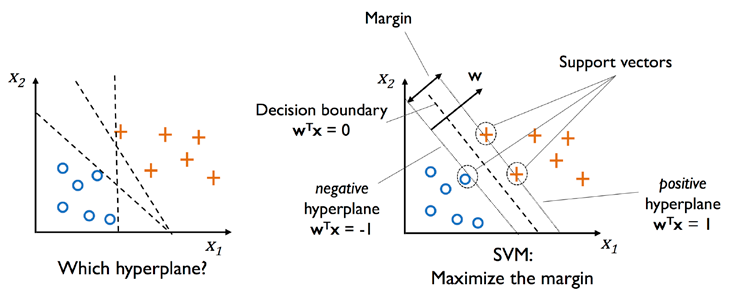
\includegraphics{./pic/chapter-4-3_pic_0.png}
\caption{image.png}
\end{figure}

    Thus SVM tries to make a decision boundary in such a way that the
separation between the two classes (the margin) is as wide as possible.

    \hypertarget{what-is-a-hyperplane}{%
\subsubsection{What is a Hyperplane?}\label{what-is-a-hyperplane}}

In geometry, it is an n-dimensional generalization of a plane, a
subspace with one less dimension \((n-1)\) than its origin space. In
one-dimensional space, it is a point, In two-dimensional space it is a
line, In three-dimensional space, it is an ordinary plane, in four or
more dimensional spaces, it is then called a `Hyperplane'. Take note of
this, it is really how the Support Vector Machine works behind the
scenes, the dimensions are the features represented in the data. For
example, say we want to carry out a classification problem and we want
to be able to tell if a product gets purchased or not(a binary
classification), if there is just one feature (say Gender) available as
a feature in the dataset, then it is in one-dimensional space and the
subspace (the separating/decision boundary) representation will be
\((n-1=0)\) a 0-dimensional space, represented with just a point showing
the separation of classes (Purchased or not). If there are two
features(Age and Gender), it is a two-dimensional space (2D), with
either of Age and Gender on the \(X\) and \(Y\)-axis, the decision
boundary will be represented as a simple line. Similarly, if the
features are three(Age, Gender, Income), the decision boundary will be a
two-dimensional plane in a three-dimensional space. Furthermore, if we
have a four or more dimensional space data points, then it is called a
`Hyperplane' with \(n-1\) dimension.

    The Hyperplane is simply a concept that separates an n-dimensional space
into two groups/halves. In machine learning terms, it is a form of a
decision boundary that algorithms like the Support Vector Machine uses
to classify or separate data points. There are two parts to it, the
negative side hyperplane and the positive part hyperplane, where data
points/instances can lie on either part, signifying the group/class they
belong to.

    \hypertarget{hard-margins}{%
\subsubsection{Hard Margins}\label{hard-margins}}

The rationale behind having decision boundaries with large margins is
that they tend to have a lower generalization error, whereas models with
small margins are more prone to overfitting. To get an idea of the
margin maximization, let's take a closer look at those positive and
negative hyperplanes that are parallel to the decision boundary.

When the data is linearly separable, and we don't want to have any
misclassifications, we use SVM with a \textbf{hard margin}. However,
when a linear boundary is not feasible, or we want to allow some
misclassifications in the hope of achieving better generality, we can
opt for a \textbf{soft margin} for our classifier.

\ldots{}

    \begin{figure}
\centering
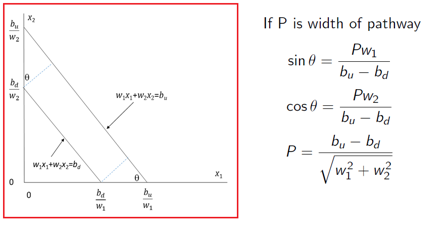
\includegraphics{./pic/chapter-4-3_pic_1.png}
\caption{chapter-4-4\_pic\_10.png}
\end{figure}

    We can scale \(w_1\), \(w_2\), \(b_u\), and \(b_d\) by the same constant
without changing the model. We can therefore set \(b_u=b+1\) and
\(b_d=b-1\) so that the width of the pathway is

\[P = \frac{2}{\sqrt{w_1^2+w_2^2}} = \frac{2}{\vert\vert \mathbf{w} \vert\vert^2}\]

In the \textbf{hard margin} case the algorithm minimizes \(w_1^2+w_2^2\)
subject to \textbf{perfect separation} being achieved

Now, the objective function of the SVM becomes the maximization of this
margin by maximizing \(P\) under the constraint that the examples are
classified correctly, which can be written as:

\[b + \mathbf{w}^𝑇 \cdot \mathbf{x}^{(𝑖)} \ge 1 \quad \text{if } 𝑦^{(𝑖)} = 1\]
\[b + \mathbf{w}^𝑇 \cdot \mathbf{x}^{(𝑖)} \le 1 \quad \text{if } 𝑦^{(𝑖)} = -1\]

for \(𝑖 = 1, \dots, 𝑁\). Here, \(N\) is the number of examples in our
dataset.

These two equations basically say that all negative-class examples
should fall on one side of the negative hyperplane, whereas all the
positive-class examples should fall behind the positive hyperplane,
which can also be written more compactly as follows:

\begin{equation}
𝑦^{(𝑖)}\left(b + \mathbf{w}^𝑇 \cdot \mathbf{x}^{(𝑖)}\right) \ge 1 \quad \forall i
\end{equation}

In practice, though, it is easier to minimize the reciprocal term,
\(\frac{1}{2}\vert\vert\mathbf{w}\vert\vert^2\) , which can be solved by
quadratic programming.

    \hypertarget{lagrange-multiplier}{%
\subsubsection{Lagrange Multiplier}\label{lagrange-multiplier}}

Because we have a contrained optimization problem (with inequality
contraints) we can recast the problem using Lagrange multipliers,
\(\alpha \ge 0\) and search for the critical points of

\begin{equation}\label{eq:7.7}
L = \frac{1}{2} \vert \theta \vert^2 - \sum\limits_{n=1}^N \alpha_n \left( y^{(n)} \left( \mathbf{\theta}^T \mathbf{x}^{(n)} + \theta_0 \right) -1 \right)
\end{equation}

To find the critical points we differentiate with respect to the scalar
\(\theta_0\) and with respect to the vector \(\mathbf{\theta}\).
Remember that differentiation with respect to a vector just means
differentiating with respect to each of its entries. Setting these
derivatives to zero you end up with:

\begin{equation}\label{eq:7.8}
\sum\limits_{n=1}^N \alpha_n  y^{(n)} = 0
\end{equation}

and

\begin{equation}\label{eq:7.9}
\mathbf{\theta} = \sum\limits_{n=1}^N \alpha_n  y^{(n)} \mathbf{x}^{(n)} 
\end{equation}

which means that our vector orthogonal to the hyperplane is just a
linear combination of sample vectors. Substituting \eqref{eq:7.9} into
\eqref{eq:7.7} and using \eqref{eq:7.8} results in

\begin{equation}
L = \sum\limits_{n=1}^N \alpha_n - \frac{1}{2} \sum\limits_{i=1}^N \sum\limits_{j=1}^N \alpha_i \alpha_j y^{(i)} 
{\mathbf{x}^{(i)}}^T \mathbf{x}^{(j)} 
\end{equation}

We want to maximize \(L\) over the \(\alpha\)s, all greater than or
equal to zero, subject to \eqref{eq:7.8}. This is known as the dual
problem.

Once we have found the \(\alpha\)s the dual version of the classifier
for a new point \(\mathbf{u}\) is the just \begin{equation}
\sum\limits_{n=1}^N \alpha_n   y^{(n)} {\mathbf{x}^{(n)}}^T  \mathbf{u} + \theta_0
\end{equation}

whether this is greater or less than zero.

\textbf{TODO Chiarire bene la seguente frase:} The maximization of \(L\)
whill return almost all \(\alpha\)s as zero. Those that aren't zero
correspond to the support vectors, the cases that define the margins.

    \hypertarget{soft-margins}{%
\subsubsection{Soft Margins}\label{soft-margins}}

    Let's briefly mention the slack variable, 𝜉𝜉 , which was introduced by
Vladimir Vapnik in 1995 and led to the socalled soft-margin
classification. The motivation for introducing the slack variable,
\(\xi\) , was that the linear constraints need to be relaxed for
nonlinearly separable data to allow the convergence of the optimization
in the presence of misclassifications, under appropriate cost
penalization.

The positive-valued slack variable is simply added to the linear
constraints:

\[b + \mathbf{w}^𝑇 \cdot \mathbf{x}^{(𝑖)} \ge 1  - \xi^{(i)}\quad \text{if } 𝑦^{(𝑖)} = 1\]

\[b + \mathbf{w}^𝑇 \cdot \mathbf{x}^{(𝑖)} \le -1  + \xi^{(i)}\quad \text{if } 𝑦^{(𝑖)} = -1\]

So, the new objective to be minimized (subject to the contraints)
becomes

\begin{equation}
\frac{1}{2} \vert\vert \mathbf{w} \vert\vert^2 + C \left( \sum_i \xi^{(i)} \right)
\end{equation}

Via the variable, C, we can then control the penalty for
misclassification. Large values of C correspond to large error
penalties, whereas we are less strict about misclassification errors if
we choose smaller values for C. We can then use the C parameter to
control the width of the margin and therefore tune the bias-variance
tradeoff.

    \begin{figure}
\centering
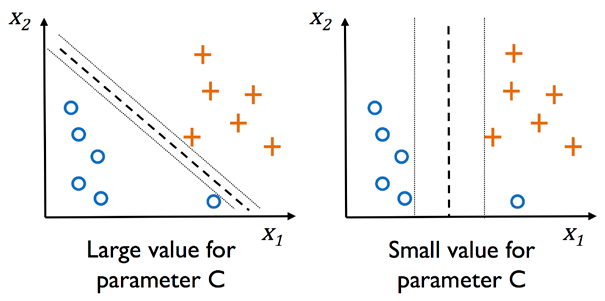
\includegraphics{./pic/chapter-4-3_pic_2.png}
\caption{image.png}
\end{figure}

    \hypertarget{example}{%
\subsection{Example}\label{example}}

    \begin{tcolorbox}[breakable, size=fbox, boxrule=1pt, pad at break*=1mm,colback=cellbackground, colframe=cellborder]
\prompt{In}{incolor}{1}{\boxspacing}
\begin{Verbatim}[commandchars=\\\{\}]
\PY{c+c1}{\PYZsh{} This section carries out calculations for the example in Table 5.2 of Chapter 5 Hull J. C.}
\end{Verbatim}
\end{tcolorbox}

    \begin{tcolorbox}[breakable, size=fbox, boxrule=1pt, pad at break*=1mm,colback=cellbackground, colframe=cellborder]
\prompt{In}{incolor}{2}{\boxspacing}
\begin{Verbatim}[commandchars=\\\{\}]
\PY{k+kn}{from} \PY{n+nn}{sklearn}\PY{n+nn}{.}\PY{n+nn}{svm} \PY{k+kn}{import} \PY{n}{LinearSVC}
\PY{k+kn}{from} \PY{n+nn}{sklearn}\PY{n+nn}{.}\PY{n+nn}{svm} \PY{k+kn}{import} \PY{n}{SVC}
\PY{k+kn}{import} \PY{n+nn}{pandas} \PY{k}{as} \PY{n+nn}{pd} 
\PY{k+kn}{import} \PY{n+nn}{numpy} \PY{k}{as} \PY{n+nn}{np}
\PY{k+kn}{import} \PY{n+nn}{matplotlib}\PY{n+nn}{.}\PY{n+nn}{pyplot} \PY{k}{as} \PY{n+nn}{plt}
\end{Verbatim}
\end{tcolorbox}

    \begin{tcolorbox}[breakable, size=fbox, boxrule=1pt, pad at break*=1mm,colback=cellbackground, colframe=cellborder]
\prompt{In}{incolor}{3}{\boxspacing}
\begin{Verbatim}[commandchars=\\\{\}]
\PY{n}{Income} \PY{o}{=} \PY{n}{pd}\PY{o}{.}\PY{n}{DataFrame}\PY{p}{(}\PY{p}{[}\PY{l+m+mi}{30}\PY{p}{,} \PY{l+m+mi}{55}\PY{p}{,} \PY{l+m+mi}{63}\PY{p}{,} \PY{l+m+mi}{35}\PY{p}{,} \PY{l+m+mi}{28}\PY{p}{,} \PY{l+m+mi}{140}\PY{p}{,} \PY{l+m+mi}{100}\PY{p}{,} \PY{l+m+mi}{95}\PY{p}{,} \PY{l+m+mi}{64}\PY{p}{,} \PY{l+m+mi}{63}\PY{p}{]}\PY{p}{)}
\PY{n}{Credit} \PY{o}{=} \PY{n}{pd}\PY{o}{.}\PY{n}{DataFrame}\PY{p}{(}\PY{p}{[}\PY{l+m+mi}{40}\PY{p}{,} \PY{l+m+mi}{30}\PY{p}{,} \PY{l+m+mi}{30}\PY{p}{,} \PY{l+m+mi}{80}\PY{p}{,} \PY{l+m+mi}{100}\PY{p}{,} \PY{l+m+mi}{30}\PY{p}{,} \PY{l+m+mi}{30}\PY{p}{,} \PY{l+m+mi}{90}\PY{p}{,} \PY{l+m+mi}{120}\PY{p}{,} \PY{l+m+mi}{150}\PY{p}{]}\PY{p}{)}
\PY{n}{Loan} \PY{o}{=} \PY{n}{pd}\PY{o}{.}\PY{n}{DataFrame}\PY{p}{(}\PY{p}{[}\PY{l+m+mi}{0}\PY{p}{,} \PY{l+m+mi}{0}\PY{p}{,} \PY{l+m+mi}{0}\PY{p}{,} \PY{l+m+mi}{0}\PY{p}{,} \PY{l+m+mi}{0}\PY{p}{,} \PY{l+m+mi}{1}\PY{p}{,} \PY{l+m+mi}{1}\PY{p}{,} \PY{l+m+mi}{1}\PY{p}{,} \PY{l+m+mi}{1}\PY{p}{,} \PY{l+m+mi}{1}\PY{p}{]}\PY{p}{)}
\end{Verbatim}
\end{tcolorbox}

    \begin{tcolorbox}[breakable, size=fbox, boxrule=1pt, pad at break*=1mm,colback=cellbackground, colframe=cellborder]
\prompt{In}{incolor}{4}{\boxspacing}
\begin{Verbatim}[commandchars=\\\{\}]
\PY{n}{plt}\PY{o}{.}\PY{n}{figure}\PY{p}{(}\PY{n}{figsize}\PY{o}{=}\PY{p}{(}\PY{l+m+mi}{10}\PY{p}{,}\PY{l+m+mi}{8}\PY{p}{)}\PY{p}{)}
\PY{n}{plt}\PY{o}{.}\PY{n}{scatter}\PY{p}{(}\PY{n}{Income}\PY{p}{,} \PY{n}{Credit}\PY{p}{,} \PY{n}{c}\PY{o}{=}\PY{n}{Loan}\PY{p}{)}
\PY{n}{plt}\PY{o}{.}\PY{n}{xlabel}\PY{p}{(}\PY{l+s+s1}{\PYZsq{}}\PY{l+s+s1}{Income}\PY{l+s+s1}{\PYZsq{}}\PY{p}{)}
\PY{n}{plt}\PY{o}{.}\PY{n}{ylabel}\PY{p}{(}\PY{l+s+s1}{\PYZsq{}}\PY{l+s+s1}{Adjusted Credit Score}\PY{l+s+s1}{\PYZsq{}}\PY{p}{)}
\PY{n}{axes} \PY{o}{=} \PY{n}{plt}\PY{o}{.}\PY{n}{gca}\PY{p}{(}\PY{p}{)}
\PY{n}{axes}\PY{o}{.}\PY{n}{set\PYZus{}xlim}\PY{p}{(}\PY{p}{[}\PY{l+m+mi}{0}\PY{p}{,}\PY{l+m+mi}{160}\PY{p}{]}\PY{p}{)}
\PY{n}{axes}\PY{o}{.}\PY{n}{set\PYZus{}ylim}\PY{p}{(}\PY{p}{[}\PY{l+m+mi}{0}\PY{p}{,}\PY{l+m+mi}{300}\PY{p}{]}\PY{p}{)}
\PY{n}{plt}\PY{o}{.}\PY{n}{show}\PY{p}{(}\PY{p}{)}
\end{Verbatim}
\end{tcolorbox}

    \begin{center}
    \adjustimage{max size={0.9\linewidth}{0.9\paperheight}}{output_21_0.png}
    \end{center}
    { \hspace*{\fill} \\}
    
    \hypertarget{hard-margin-calculation}{%
\subsubsection{Hard Margin Calculation}\label{hard-margin-calculation}}

    \begin{tcolorbox}[breakable, size=fbox, boxrule=1pt, pad at break*=1mm,colback=cellbackground, colframe=cellborder]
\prompt{In}{incolor}{5}{\boxspacing}
\begin{Verbatim}[commandchars=\\\{\}]
\PY{n}{X} \PY{o}{=} \PY{n}{np}\PY{o}{.}\PY{n}{asarray}\PY{p}{(}\PY{n}{pd}\PY{o}{.}\PY{n}{concat}\PY{p}{(}\PY{p}{[}\PY{n}{Income}\PY{p}{,} \PY{n}{Credit}\PY{p}{]}\PY{p}{,}\PY{n}{axis}\PY{o}{=}\PY{l+m+mi}{1}\PY{p}{)}\PY{p}{)}
\PY{n}{y} \PY{o}{=} \PY{n}{np}\PY{o}{.}\PY{n}{asarray}\PY{p}{(}\PY{n}{Loan}\PY{p}{)}\PY{o}{.}\PY{n}{ravel}\PY{p}{(}\PY{p}{)}
\PY{n}{clf} \PY{o}{=} \PY{n}{SVC}\PY{p}{(}\PY{n}{kernel}\PY{o}{=}\PY{l+s+s1}{\PYZsq{}}\PY{l+s+s1}{linear}\PY{l+s+s1}{\PYZsq{}}\PY{p}{,}\PY{n}{tol}\PY{o}{=}\PY{l+m+mf}{1e\PYZhy{}5}\PY{p}{)}
\PY{n}{clf}\PY{o}{.}\PY{n}{fit}\PY{p}{(}\PY{n}{X}\PY{p}{,}\PY{n}{y}\PY{p}{)}
\end{Verbatim}
\end{tcolorbox}

            \begin{tcolorbox}[breakable, size=fbox, boxrule=.5pt, pad at break*=1mm, opacityfill=0]
\prompt{Out}{outcolor}{5}{\boxspacing}
\begin{Verbatim}[commandchars=\\\{\}]
SVC(kernel='linear', tol=1e-05)
\end{Verbatim}
\end{tcolorbox}
        
    \begin{tcolorbox}[breakable, size=fbox, boxrule=1pt, pad at break*=1mm,colback=cellbackground, colframe=cellborder]
\prompt{In}{incolor}{6}{\boxspacing}
\begin{Verbatim}[commandchars=\\\{\}]
\PY{n}{w} \PY{o}{=} \PY{n}{clf}\PY{o}{.}\PY{n}{coef\PYZus{}}\PY{p}{[}\PY{l+m+mi}{0}\PY{p}{]}
\PY{n}{b} \PY{o}{=} \PY{o}{\PYZhy{}}\PY{n}{clf}\PY{o}{.}\PY{n}{intercept\PYZus{}}\PY{p}{[}\PY{l+m+mi}{0}\PY{p}{]}
\PY{n+nb}{print}\PY{p}{(}\PY{n}{w}\PY{p}{)}
\PY{n+nb}{print}\PY{p}{(}\PY{n}{b}\PY{p}{)}
\end{Verbatim}
\end{tcolorbox}

    \begin{Verbatim}[commandchars=\\\{\}]
[0.05405405 0.02162159]
5.054052228526239
    \end{Verbatim}

    The outer lines are \(w_1x_1+w_2x_2 = b_u\) and \(w_1x_1+w_2x_2=b_d\).
The middle line is \(w_1x_1+w_2x_2=b\), where \(b_u=b+1\) and
\(b_d=b-1\). The width of the path is \(\frac{2}{\sqrt{w_1^2+w_2^2}}\).

    \begin{tcolorbox}[breakable, size=fbox, boxrule=1pt, pad at break*=1mm,colback=cellbackground, colframe=cellborder]
\prompt{In}{incolor}{7}{\boxspacing}
\begin{Verbatim}[commandchars=\\\{\}]
\PY{n}{x1} \PY{o}{=} \PY{n}{np}\PY{o}{.}\PY{n}{linspace}\PY{p}{(}\PY{l+m+mi}{0}\PY{p}{,}\PY{l+m+mi}{160}\PY{p}{,}\PY{l+m+mi}{300}\PY{p}{)}
\PY{n}{w1} \PY{o}{=} \PY{n}{w}\PY{p}{[}\PY{l+m+mi}{0}\PY{p}{]}
\PY{n}{w2} \PY{o}{=} \PY{n}{w}\PY{p}{[}\PY{l+m+mi}{1}\PY{p}{]}
\PY{n}{bu} \PY{o}{=} \PY{n}{b}\PY{o}{+}\PY{l+m+mi}{1}
\PY{n}{bd} \PY{o}{=} \PY{n}{b}\PY{o}{\PYZhy{}}\PY{l+m+mi}{1}
\PY{n}{y1} \PY{o}{=} \PY{p}{(}\PY{n}{bu}\PY{o}{\PYZhy{}}\PY{n}{w1}\PY{o}{*}\PY{n}{x1}\PY{p}{)}\PY{o}{/}\PY{n}{w2}
\PY{n}{y2} \PY{o}{=} \PY{p}{(}\PY{n}{bd}\PY{o}{\PYZhy{}}\PY{n}{w1}\PY{o}{*}\PY{n}{x1}\PY{p}{)}\PY{o}{/}\PY{n}{w2}
\PY{n}{y0} \PY{o}{=} \PY{p}{(}\PY{n}{b}\PY{o}{\PYZhy{}}\PY{n}{w1}\PY{o}{*}\PY{n}{x1}\PY{p}{)}\PY{o}{/}\PY{n}{w2}
\PY{n}{plt}\PY{o}{.}\PY{n}{figure}\PY{p}{(}\PY{n}{figsize}\PY{o}{=}\PY{p}{(}\PY{l+m+mi}{10}\PY{p}{,}\PY{l+m+mi}{8}\PY{p}{)}\PY{p}{)}
\PY{n}{plt}\PY{o}{.}\PY{n}{scatter}\PY{p}{(}\PY{n}{Income}\PY{p}{,} \PY{n}{Credit}\PY{p}{,} \PY{n}{c}\PY{o}{=}\PY{n}{Loan}\PY{p}{)}
\PY{n}{plt}\PY{o}{.}\PY{n}{plot}\PY{p}{(}\PY{n}{x1}\PY{p}{,}\PY{n}{y1}\PY{p}{,}\PY{l+s+s1}{\PYZsq{}}\PY{l+s+s1}{\PYZhy{}\PYZhy{}}\PY{l+s+s1}{\PYZsq{}}\PY{p}{,}\PY{n}{color}\PY{o}{=}\PY{l+s+s1}{\PYZsq{}}\PY{l+s+s1}{skyblue}\PY{l+s+s1}{\PYZsq{}}\PY{p}{)}
\PY{n}{plt}\PY{o}{.}\PY{n}{plot}\PY{p}{(}\PY{n}{x1}\PY{p}{,}\PY{n}{y2}\PY{p}{,}\PY{l+s+s1}{\PYZsq{}}\PY{l+s+s1}{\PYZhy{}\PYZhy{}}\PY{l+s+s1}{\PYZsq{}}\PY{p}{,}\PY{n}{color}\PY{o}{=}\PY{l+s+s1}{\PYZsq{}}\PY{l+s+s1}{skyblue}\PY{l+s+s1}{\PYZsq{}}\PY{p}{)}
\PY{n}{plt}\PY{o}{.}\PY{n}{plot}\PY{p}{(}\PY{n}{x1}\PY{p}{,}\PY{n}{y0}\PY{p}{,}\PY{l+s+s1}{\PYZsq{}}\PY{l+s+s1}{\PYZhy{}}\PY{l+s+s1}{\PYZsq{}}\PY{p}{)}
\PY{n}{plt}\PY{o}{.}\PY{n}{xlabel}\PY{p}{(}\PY{l+s+s1}{\PYZsq{}}\PY{l+s+s1}{Income}\PY{l+s+s1}{\PYZsq{}}\PY{p}{)}
\PY{n}{plt}\PY{o}{.}\PY{n}{ylabel}\PY{p}{(}\PY{l+s+s1}{\PYZsq{}}\PY{l+s+s1}{Adjusted Credit Score}\PY{l+s+s1}{\PYZsq{}}\PY{p}{)}
\PY{n}{axes} \PY{o}{=} \PY{n}{plt}\PY{o}{.}\PY{n}{gca}\PY{p}{(}\PY{p}{)}
\PY{n}{axes}\PY{o}{.}\PY{n}{set\PYZus{}xlim}\PY{p}{(}\PY{p}{[}\PY{l+m+mi}{0}\PY{p}{,}\PY{l+m+mi}{160}\PY{p}{]}\PY{p}{)}
\PY{n}{axes}\PY{o}{.}\PY{n}{set\PYZus{}ylim}\PY{p}{(}\PY{p}{[}\PY{l+m+mi}{0}\PY{p}{,} \PY{l+m+mi}{350}\PY{p}{]}\PY{p}{)}
\PY{n}{plt}\PY{o}{.}\PY{n}{show}\PY{p}{(}\PY{p}{)}
\end{Verbatim}
\end{tcolorbox}

    \begin{center}
    \adjustimage{max size={0.9\linewidth}{0.9\paperheight}}{output_26_0.png}
    \end{center}
    { \hspace*{\fill} \\}
    
    \hypertarget{modification-for-soft-margin}{%
\subsubsection{Modification for Soft
Margin}\label{modification-for-soft-margin}}

    Note that the objective function of SVC is
\(C\sum_{j=1}^n z_j+\frac{1}{2}\sum_{j=1}^nw_j^2\). If our objective
function is \(C\sum_{j=1}^n z_j+\sum_{j=1}^nw_j^2\), then we to set
\(C=C/2\) in SVC.

    \begin{tcolorbox}[breakable, size=fbox, boxrule=1pt, pad at break*=1mm,colback=cellbackground, colframe=cellborder]
\prompt{In}{incolor}{8}{\boxspacing}
\begin{Verbatim}[commandchars=\\\{\}]
\PY{c+c1}{\PYZsh{}We carry out calculations for C=0.0005 which corresponds to C=0.001 in Hull\PYZsq{}s book. }
\PY{n}{X} \PY{o}{=} \PY{n}{np}\PY{o}{.}\PY{n}{asarray}\PY{p}{(}\PY{n}{pd}\PY{o}{.}\PY{n}{concat}\PY{p}{(}\PY{p}{[}\PY{n}{Income}\PY{p}{,} \PY{n}{Credit}\PY{p}{]}\PY{p}{,}\PY{n}{axis}\PY{o}{=}\PY{l+m+mi}{1}\PY{p}{)}\PY{p}{)}
\PY{n}{y} \PY{o}{=} \PY{n}{np}\PY{o}{.}\PY{n}{asarray}\PY{p}{(}\PY{n}{Loan}\PY{p}{)}\PY{o}{.}\PY{n}{ravel}\PY{p}{(}\PY{p}{)}
\PY{n}{clf} \PY{o}{=} \PY{n}{SVC}\PY{p}{(}\PY{n}{kernel}\PY{o}{=}\PY{l+s+s1}{\PYZsq{}}\PY{l+s+s1}{linear}\PY{l+s+s1}{\PYZsq{}}\PY{p}{,}\PY{n}{C}\PY{o}{=}\PY{l+m+mf}{0.0005}\PY{p}{,}\PY{n}{tol}\PY{o}{=}\PY{l+m+mf}{1e\PYZhy{}5}\PY{p}{)}
\PY{n}{clf}\PY{o}{.}\PY{n}{fit}\PY{p}{(}\PY{n}{X}\PY{p}{,}\PY{n}{y}\PY{p}{)}
\end{Verbatim}
\end{tcolorbox}

            \begin{tcolorbox}[breakable, size=fbox, boxrule=.5pt, pad at break*=1mm, opacityfill=0]
\prompt{Out}{outcolor}{8}{\boxspacing}
\begin{Verbatim}[commandchars=\\\{\}]
SVC(C=0.0005, kernel='linear', tol=1e-05)
\end{Verbatim}
\end{tcolorbox}
        
    \begin{tcolorbox}[breakable, size=fbox, boxrule=1pt, pad at break*=1mm,colback=cellbackground, colframe=cellborder]
\prompt{In}{incolor}{9}{\boxspacing}
\begin{Verbatim}[commandchars=\\\{\}]
\PY{n}{w} \PY{o}{=} \PY{n}{clf}\PY{o}{.}\PY{n}{coef\PYZus{}}\PY{p}{[}\PY{l+m+mi}{0}\PY{p}{]}
\PY{n}{b} \PY{o}{=} \PY{o}{\PYZhy{}}\PY{n}{clf}\PY{o}{.}\PY{n}{intercept\PYZus{}}\PY{p}{[}\PY{l+m+mi}{0}\PY{p}{]}
\PY{n+nb}{print}\PY{p}{(}\PY{n}{w}\PY{p}{)}
\PY{n+nb}{print}\PY{p}{(}\PY{n}{b}\PY{p}{)}
\end{Verbatim}
\end{tcolorbox}

    \begin{Verbatim}[commandchars=\\\{\}]
[0.03678097 0.0142146 ]
3.449391592920354
    \end{Verbatim}

    The outer lines are \(w_1x_1+w_2x_2 = b_u\) and \(w_1x_1+w_2x_2=b_d\).
The middle line is \(w_1x_1+w_2x_2=b\), where \(b_u=b+1\) and
\(b_d=b-1\). The width of the path is \(\frac{2}{\sqrt{w_1^2+w_2^2}}\).

    \begin{tcolorbox}[breakable, size=fbox, boxrule=1pt, pad at break*=1mm,colback=cellbackground, colframe=cellborder]
\prompt{In}{incolor}{10}{\boxspacing}
\begin{Verbatim}[commandchars=\\\{\}]
\PY{n}{x1} \PY{o}{=} \PY{n}{np}\PY{o}{.}\PY{n}{linspace}\PY{p}{(}\PY{l+m+mi}{0}\PY{p}{,}\PY{l+m+mi}{160}\PY{p}{,}\PY{l+m+mi}{100}\PY{p}{)}
\PY{n}{w1} \PY{o}{=} \PY{n}{w}\PY{p}{[}\PY{l+m+mi}{0}\PY{p}{]}
\PY{n}{w2} \PY{o}{=} \PY{n}{w}\PY{p}{[}\PY{l+m+mi}{1}\PY{p}{]}
\PY{n}{bu} \PY{o}{=} \PY{n}{b}\PY{o}{+}\PY{l+m+mi}{1}
\PY{n}{bd} \PY{o}{=} \PY{n}{b}\PY{o}{\PYZhy{}}\PY{l+m+mi}{1}
\PY{n}{y1} \PY{o}{=} \PY{p}{(}\PY{n}{bu}\PY{o}{\PYZhy{}}\PY{n}{w1}\PY{o}{*}\PY{n}{x1}\PY{p}{)}\PY{o}{/}\PY{n}{w2}
\PY{n}{y2} \PY{o}{=} \PY{p}{(}\PY{n}{bd}\PY{o}{\PYZhy{}}\PY{n}{w1}\PY{o}{*}\PY{n}{x1}\PY{p}{)}\PY{o}{/}\PY{n}{w2}
\PY{n}{y0} \PY{o}{=} \PY{p}{(}\PY{n}{b}\PY{o}{\PYZhy{}}\PY{n}{w1}\PY{o}{*}\PY{n}{x1}\PY{p}{)}\PY{o}{/}\PY{n}{w2}
\PY{n}{plt}\PY{o}{.}\PY{n}{figure}\PY{p}{(}\PY{n}{figsize}\PY{o}{=}\PY{p}{(}\PY{l+m+mi}{10}\PY{p}{,}\PY{l+m+mi}{8}\PY{p}{)}\PY{p}{)}
\PY{n}{plt}\PY{o}{.}\PY{n}{scatter}\PY{p}{(}\PY{n}{Income}\PY{p}{,} \PY{n}{Credit}\PY{p}{,} \PY{n}{c}\PY{o}{=}\PY{n}{Loan}\PY{p}{)}
\PY{n}{plt}\PY{o}{.}\PY{n}{plot}\PY{p}{(}\PY{n}{x1}\PY{p}{,}\PY{n}{y1}\PY{p}{,}\PY{l+s+s1}{\PYZsq{}}\PY{l+s+s1}{\PYZhy{}\PYZhy{}}\PY{l+s+s1}{\PYZsq{}}\PY{p}{,}\PY{n}{color}\PY{o}{=}\PY{l+s+s1}{\PYZsq{}}\PY{l+s+s1}{skyblue}\PY{l+s+s1}{\PYZsq{}}\PY{p}{)}
\PY{n}{plt}\PY{o}{.}\PY{n}{plot}\PY{p}{(}\PY{n}{x1}\PY{p}{,}\PY{n}{y2}\PY{p}{,}\PY{l+s+s1}{\PYZsq{}}\PY{l+s+s1}{\PYZhy{}\PYZhy{}}\PY{l+s+s1}{\PYZsq{}}\PY{p}{,}\PY{n}{color}\PY{o}{=}\PY{l+s+s1}{\PYZsq{}}\PY{l+s+s1}{skyblue}\PY{l+s+s1}{\PYZsq{}}\PY{p}{)}
\PY{n}{plt}\PY{o}{.}\PY{n}{plot}\PY{p}{(}\PY{n}{x1}\PY{p}{,}\PY{n}{y0}\PY{p}{,}\PY{l+s+s1}{\PYZsq{}}\PY{l+s+s1}{\PYZhy{}}\PY{l+s+s1}{\PYZsq{}}\PY{p}{)}
\PY{n}{plt}\PY{o}{.}\PY{n}{xlabel}\PY{p}{(}\PY{l+s+s1}{\PYZsq{}}\PY{l+s+s1}{Income}\PY{l+s+s1}{\PYZsq{}}\PY{p}{)}
\PY{n}{plt}\PY{o}{.}\PY{n}{ylabel}\PY{p}{(}\PY{l+s+s1}{\PYZsq{}}\PY{l+s+s1}{Adjusted Credit Score}\PY{l+s+s1}{\PYZsq{}}\PY{p}{)}
\PY{n}{axes} \PY{o}{=} \PY{n}{plt}\PY{o}{.}\PY{n}{gca}\PY{p}{(}\PY{p}{)}
\PY{n}{axes}\PY{o}{.}\PY{n}{set\PYZus{}xlim}\PY{p}{(}\PY{p}{[}\PY{l+m+mi}{0}\PY{p}{,}\PY{l+m+mi}{160}\PY{p}{]}\PY{p}{)}
\PY{n}{axes}\PY{o}{.}\PY{n}{set\PYZus{}ylim}\PY{p}{(}\PY{p}{[}\PY{l+m+mi}{0}\PY{p}{,} \PY{l+m+mi}{350}\PY{p}{]}\PY{p}{)}
\PY{n}{plt}\PY{o}{.}\PY{n}{show}\PY{p}{(}\PY{p}{)}
\end{Verbatim}
\end{tcolorbox}

    \begin{center}
    \adjustimage{max size={0.9\linewidth}{0.9\paperheight}}{output_32_0.png}
    \end{center}
    { \hspace*{\fill} \\}
    
    For different values of \(C\) and find out the loans misclassified as
well as width of pathway

    \begin{tcolorbox}[breakable, size=fbox, boxrule=1pt, pad at break*=1mm,colback=cellbackground, colframe=cellborder]
\prompt{In}{incolor}{11}{\boxspacing}
\begin{Verbatim}[commandchars=\\\{\}]
\PY{c+c1}{\PYZsh{} The values of C are those in Hull\PYZsq{}s book. We divide them by 2 to get corresponding values for Sklearn}
\PY{k}{for} \PY{n}{C} \PY{o+ow}{in} \PY{p}{[}\PY{l+m+mf}{0.01}\PY{p}{,} \PY{l+m+mf}{0.001}\PY{p}{,} \PY{l+m+mf}{0.0005}\PY{p}{,} \PY{l+m+mf}{0.0003}\PY{p}{,} \PY{l+m+mf}{0.0002}\PY{p}{]}\PY{p}{:}
    \PY{n}{clf} \PY{o}{=} \PY{n}{SVC}\PY{p}{(}\PY{n}{kernel}\PY{o}{=}\PY{l+s+s1}{\PYZsq{}}\PY{l+s+s1}{linear}\PY{l+s+s1}{\PYZsq{}}\PY{p}{,}\PY{n}{C}\PY{o}{=}\PY{n}{C}\PY{o}{/}\PY{l+m+mi}{2}\PY{p}{,}\PY{n}{tol}\PY{o}{=}\PY{l+m+mf}{1e\PYZhy{}6}\PY{p}{)}
    \PY{n}{clf}\PY{o}{.}\PY{n}{fit}\PY{p}{(}\PY{n}{X}\PY{p}{,}\PY{n}{y}\PY{p}{)}
    \PY{n}{S} \PY{o}{=} \PY{n}{clf}\PY{o}{.}\PY{n}{score}\PY{p}{(}\PY{n}{X}\PY{p}{,}\PY{n}{y}\PY{p}{)}
    \PY{n}{w} \PY{o}{=} \PY{n}{clf}\PY{o}{.}\PY{n}{coef\PYZus{}}\PY{p}{[}\PY{l+m+mi}{0}\PY{p}{]}
    \PY{n}{b} \PY{o}{=} \PY{o}{\PYZhy{}}\PY{n}{clf}\PY{o}{.}\PY{n}{intercept\PYZus{}}\PY{p}{[}\PY{l+m+mi}{0}\PY{p}{]}
    \PY{n}{P} \PY{o}{=} \PY{l+m+mi}{2}\PY{o}{/}\PY{n}{np}\PY{o}{.}\PY{n}{sqrt}\PY{p}{(}\PY{n}{w}\PY{p}{[}\PY{l+m+mi}{0}\PY{p}{]}\PY{o}{*}\PY{o}{*}\PY{l+m+mi}{2}\PY{o}{+}\PY{n}{w}\PY{p}{[}\PY{l+m+mi}{1}\PY{p}{]}\PY{o}{*}\PY{o}{*}\PY{l+m+mi}{2}\PY{p}{)}
    \PY{n+nb}{sum} \PY{o}{=} \PY{l+m+mi}{0}
    \PY{k}{for} \PY{n}{i} \PY{o+ow}{in} \PY{n+nb}{range}\PY{p}{(}\PY{n+nb}{len}\PY{p}{(}\PY{n}{Income}\PY{p}{)}\PY{p}{)}\PY{p}{:}
        \PY{k}{if} \PY{n}{Loan}\PY{o}{.}\PY{n}{iloc}\PY{p}{[}\PY{n}{i}\PY{p}{,}\PY{l+m+mi}{0}\PY{p}{]} \PY{o}{==} \PY{l+m+mi}{0}\PY{p}{:}
            \PY{n+nb}{sum} \PY{o}{+}\PY{o}{=} \PY{n+nb}{max}\PY{p}{(}\PY{n}{w}\PY{p}{[}\PY{l+m+mi}{0}\PY{p}{]} \PY{o}{*} \PY{n}{Income}\PY{o}{.}\PY{n}{iloc}\PY{p}{[}\PY{n}{i}\PY{p}{,}\PY{l+m+mi}{0}\PY{p}{]} \PY{o}{+} \PY{n}{w}\PY{p}{[}\PY{l+m+mi}{1}\PY{p}{]} \PY{o}{*} \PY{n}{Credit}\PY{o}{.}\PY{n}{iloc}\PY{p}{[}\PY{n}{i}\PY{p}{,}\PY{l+m+mi}{0}\PY{p}{]} \PY{o}{\PYZhy{}} \PY{n}{b}\PY{p}{,}\PY{l+m+mi}{0}\PY{p}{)}
        \PY{k}{else}\PY{p}{:}
            \PY{n+nb}{sum} \PY{o}{+}\PY{o}{=} \PY{n+nb}{max}\PY{p}{(}\PY{n}{b}\PY{o}{\PYZhy{}} \PY{n}{w}\PY{p}{[}\PY{l+m+mi}{0}\PY{p}{]} \PY{o}{*} \PY{n}{Income}\PY{o}{.}\PY{n}{iloc}\PY{p}{[}\PY{n}{i}\PY{p}{,}\PY{l+m+mi}{0}\PY{p}{]} \PY{o}{\PYZhy{}} \PY{n}{w}\PY{p}{[}\PY{l+m+mi}{1}\PY{p}{]} \PY{o}{*} \PY{n}{Credit}\PY{o}{.}\PY{n}{iloc}\PY{p}{[}\PY{n}{i}\PY{p}{,}\PY{l+m+mi}{0}\PY{p}{]}\PY{p}{,}\PY{l+m+mi}{0}\PY{p}{)}
    \PY{n+nb}{print}\PY{p}{(}\PY{l+s+s2}{\PYZdq{}}\PY{l+s+s2}{C = }\PY{l+s+si}{\PYZpc{}6.4f}\PY{l+s+s2}{, w1 = }\PY{l+s+si}{\PYZpc{}6.4f}\PY{l+s+s2}{, w2 = }\PY{l+s+si}{\PYZpc{}6.4f}\PY{l+s+s2}{, b = }\PY{l+s+si}{\PYZpc{}5.2f}\PY{l+s+s2}{, Loan Misclassified = }\PY{l+s+si}{\PYZpc{}3.0f}\PY{l+s+si}{\PYZpc{}\PYZpc{}}\PY{l+s+s2}{, Width = }\PY{l+s+si}{\PYZpc{}5.1f}\PY{l+s+s2}{, Cent Error = }\PY{l+s+si}{\PYZpc{}6.4f}\PY{l+s+s2}{\PYZdq{}} \PY{o}{\PYZpc{}}\PY{p}{(}\PY{n}{C}\PY{p}{,}\PY{n}{w}\PY{p}{[}\PY{l+m+mi}{0}\PY{p}{]}\PY{p}{,}\PY{n}{w}\PY{p}{[}\PY{l+m+mi}{1}\PY{p}{]}\PY{p}{,}\PY{n}{b}\PY{p}{,}\PY{l+m+mi}{100}\PY{o}{*}\PY{p}{(}\PY{l+m+mi}{1}\PY{o}{\PYZhy{}}\PY{n}{S}\PY{p}{)}\PY{p}{,}\PY{n}{P}\PY{p}{,}\PY{n+nb}{sum}\PY{p}{)}\PY{p}{)}
\end{Verbatim}
\end{tcolorbox}

    \begin{Verbatim}[commandchars=\\\{\}]
C = 0.0100, w1 = 0.0541, w2 = 0.0216, b =  5.05, Loan Misclassified =   0\%,
Width =  34.4, Cent Error = 0.0000
C = 0.0010, w1 = 0.0368, w2 = 0.0142, b =  3.45, Loan Misclassified =   0\%,
Width =  50.7, Cent Error = 0.0000
C = 0.0005, w1 = 0.0290, w2 = 0.0155, b =  3.15, Loan Misclassified =   0\%,
Width =  60.9, Cent Error = 0.0000
C = 0.0003, w1 = 0.0235, w2 = 0.0151, b =  2.75, Loan Misclassified =   0\%,
Width =  71.5, Cent Error = 0.0000
C = 0.0002, w1 = 0.0193, w2 = 0.0124, b =  2.07, Loan Misclassified =   0\%,
Width =  87.2, Cent Error = 0.0000
    \end{Verbatim}

    \begin{tcolorbox}[breakable, size=fbox, boxrule=1pt, pad at break*=1mm,colback=cellbackground, colframe=cellborder]
\prompt{In}{incolor}{12}{\boxspacing}
\begin{Verbatim}[commandchars=\\\{\}]
\PY{c+c1}{\PYZsh{}We carry out calculations for C=0.00015 which corresponds to C=0.0003 in Hull\PYZsq{}s book. }
\PY{n}{X} \PY{o}{=} \PY{n}{np}\PY{o}{.}\PY{n}{asarray}\PY{p}{(}\PY{n}{pd}\PY{o}{.}\PY{n}{concat}\PY{p}{(}\PY{p}{[}\PY{n}{Income}\PY{p}{,} \PY{n}{Credit}\PY{p}{]}\PY{p}{,}\PY{n}{axis}\PY{o}{=}\PY{l+m+mi}{1}\PY{p}{)}\PY{p}{)}
\PY{n}{y} \PY{o}{=} \PY{n}{np}\PY{o}{.}\PY{n}{asarray}\PY{p}{(}\PY{n}{Loan}\PY{p}{)}\PY{o}{.}\PY{n}{ravel}\PY{p}{(}\PY{p}{)}
\PY{n}{clf} \PY{o}{=} \PY{n}{SVC}\PY{p}{(}\PY{n}{kernel}\PY{o}{=}\PY{l+s+s1}{\PYZsq{}}\PY{l+s+s1}{linear}\PY{l+s+s1}{\PYZsq{}}\PY{p}{,}\PY{n}{C}\PY{o}{=}\PY{l+m+mf}{0.00015}\PY{p}{,}\PY{n}{tol}\PY{o}{=}\PY{l+m+mf}{1e\PYZhy{}5}\PY{p}{)}
\PY{n}{clf}\PY{o}{.}\PY{n}{fit}\PY{p}{(}\PY{n}{X}\PY{p}{,}\PY{n}{y}\PY{p}{)}
\end{Verbatim}
\end{tcolorbox}

            \begin{tcolorbox}[breakable, size=fbox, boxrule=.5pt, pad at break*=1mm, opacityfill=0]
\prompt{Out}{outcolor}{12}{\boxspacing}
\begin{Verbatim}[commandchars=\\\{\}]
SVC(C=0.00015, kernel='linear', tol=1e-05)
\end{Verbatim}
\end{tcolorbox}
        
    \begin{tcolorbox}[breakable, size=fbox, boxrule=1pt, pad at break*=1mm,colback=cellbackground, colframe=cellborder]
\prompt{In}{incolor}{13}{\boxspacing}
\begin{Verbatim}[commandchars=\\\{\}]
\PY{n}{w} \PY{o}{=} \PY{n}{clf}\PY{o}{.}\PY{n}{coef\PYZus{}}\PY{p}{[}\PY{l+m+mi}{0}\PY{p}{]}
\PY{n}{b} \PY{o}{=} \PY{o}{\PYZhy{}}\PY{n}{clf}\PY{o}{.}\PY{n}{intercept\PYZus{}}\PY{p}{[}\PY{l+m+mi}{0}\PY{p}{]}
\PY{n+nb}{print}\PY{p}{(}\PY{n}{w}\PY{p}{)}
\PY{n+nb}{print}\PY{p}{(}\PY{n}{b}\PY{p}{)}
\end{Verbatim}
\end{tcolorbox}

    \begin{Verbatim}[commandchars=\\\{\}]
[0.02352936 0.015098  ]
2.7470513941588437
    \end{Verbatim}

    \begin{tcolorbox}[breakable, size=fbox, boxrule=1pt, pad at break*=1mm,colback=cellbackground, colframe=cellborder]
\prompt{In}{incolor}{14}{\boxspacing}
\begin{Verbatim}[commandchars=\\\{\}]
\PY{n}{x1} \PY{o}{=} \PY{n}{np}\PY{o}{.}\PY{n}{linspace}\PY{p}{(}\PY{l+m+mi}{0}\PY{p}{,}\PY{l+m+mi}{160}\PY{p}{,}\PY{l+m+mi}{100}\PY{p}{)}
\PY{n}{w1} \PY{o}{=} \PY{n}{w}\PY{p}{[}\PY{l+m+mi}{0}\PY{p}{]}
\PY{n}{w2} \PY{o}{=} \PY{n}{w}\PY{p}{[}\PY{l+m+mi}{1}\PY{p}{]}
\PY{n}{bu} \PY{o}{=} \PY{n}{b}\PY{o}{+}\PY{l+m+mi}{1}
\PY{n}{bd} \PY{o}{=} \PY{n}{b}\PY{o}{\PYZhy{}}\PY{l+m+mi}{1}
\PY{n}{y1} \PY{o}{=} \PY{p}{(}\PY{n}{bu}\PY{o}{\PYZhy{}}\PY{n}{w1}\PY{o}{*}\PY{n}{x1}\PY{p}{)}\PY{o}{/}\PY{n}{w2}
\PY{n}{y2} \PY{o}{=} \PY{p}{(}\PY{n}{bd}\PY{o}{\PYZhy{}}\PY{n}{w1}\PY{o}{*}\PY{n}{x1}\PY{p}{)}\PY{o}{/}\PY{n}{w2}
\PY{n}{y0} \PY{o}{=} \PY{p}{(}\PY{n}{b}\PY{o}{\PYZhy{}}\PY{n}{w1}\PY{o}{*}\PY{n}{x1}\PY{p}{)}\PY{o}{/}\PY{n}{w2}
\PY{n}{plt}\PY{o}{.}\PY{n}{figure}\PY{p}{(}\PY{n}{figsize}\PY{o}{=}\PY{p}{(}\PY{l+m+mi}{10}\PY{p}{,}\PY{l+m+mi}{8}\PY{p}{)}\PY{p}{)}
\PY{n}{plt}\PY{o}{.}\PY{n}{scatter}\PY{p}{(}\PY{n}{Income}\PY{p}{,} \PY{n}{Credit}\PY{p}{,} \PY{n}{c}\PY{o}{=}\PY{n}{Loan}\PY{p}{)}
\PY{n}{plt}\PY{o}{.}\PY{n}{plot}\PY{p}{(}\PY{n}{x1}\PY{p}{,}\PY{n}{y1}\PY{p}{,}\PY{l+s+s1}{\PYZsq{}}\PY{l+s+s1}{\PYZhy{}\PYZhy{}}\PY{l+s+s1}{\PYZsq{}}\PY{p}{,}\PY{n}{color}\PY{o}{=}\PY{l+s+s1}{\PYZsq{}}\PY{l+s+s1}{skyblue}\PY{l+s+s1}{\PYZsq{}}\PY{p}{)}
\PY{n}{plt}\PY{o}{.}\PY{n}{plot}\PY{p}{(}\PY{n}{x1}\PY{p}{,}\PY{n}{y2}\PY{p}{,}\PY{l+s+s1}{\PYZsq{}}\PY{l+s+s1}{\PYZhy{}\PYZhy{}}\PY{l+s+s1}{\PYZsq{}}\PY{p}{,}\PY{n}{color}\PY{o}{=}\PY{l+s+s1}{\PYZsq{}}\PY{l+s+s1}{skyblue}\PY{l+s+s1}{\PYZsq{}}\PY{p}{)}
\PY{n}{plt}\PY{o}{.}\PY{n}{plot}\PY{p}{(}\PY{n}{x1}\PY{p}{,}\PY{n}{y0}\PY{p}{,}\PY{l+s+s1}{\PYZsq{}}\PY{l+s+s1}{\PYZhy{}}\PY{l+s+s1}{\PYZsq{}}\PY{p}{)}
\PY{n}{plt}\PY{o}{.}\PY{n}{xlabel}\PY{p}{(}\PY{l+s+s1}{\PYZsq{}}\PY{l+s+s1}{Income}\PY{l+s+s1}{\PYZsq{}}\PY{p}{)}
\PY{n}{plt}\PY{o}{.}\PY{n}{ylabel}\PY{p}{(}\PY{l+s+s1}{\PYZsq{}}\PY{l+s+s1}{Adjusted Credit Score}\PY{l+s+s1}{\PYZsq{}}\PY{p}{)}
\PY{n}{axes} \PY{o}{=} \PY{n}{plt}\PY{o}{.}\PY{n}{gca}\PY{p}{(}\PY{p}{)}
\PY{n}{axes}\PY{o}{.}\PY{n}{set\PYZus{}xlim}\PY{p}{(}\PY{p}{[}\PY{l+m+mi}{0}\PY{p}{,}\PY{l+m+mi}{160}\PY{p}{]}\PY{p}{)}
\PY{n}{axes}\PY{o}{.}\PY{n}{set\PYZus{}ylim}\PY{p}{(}\PY{p}{[}\PY{l+m+mi}{0}\PY{p}{,} \PY{l+m+mi}{350}\PY{p}{]}\PY{p}{)}
\PY{n}{plt}\PY{o}{.}\PY{n}{show}\PY{p}{(}\PY{p}{)}
\end{Verbatim}
\end{tcolorbox}

    \begin{center}
    \adjustimage{max size={0.9\linewidth}{0.9\paperheight}}{output_37_0.png}
    \end{center}
    { \hspace*{\fill} \\}
    
    \begin{tcolorbox}[breakable, size=fbox, boxrule=1pt, pad at break*=1mm,colback=cellbackground, colframe=cellborder]
\prompt{In}{incolor}{ }{\boxspacing}
\begin{Verbatim}[commandchars=\\\{\}]

\end{Verbatim}
\end{tcolorbox}

    \hypertarget{non-linear-classification}{%
\subsection{Non Linear Classification}\label{non-linear-classification}}

    Another reason why SVMs enjoy high popularity among machine learning
practitioners is that they can be easily kernelized to solve nonlinear
classification problems. Before we discuss the main concept behind the
so-called kernel SVM, the most common variant of SVMs, let's first
create a synthetic dataset to see what such a nonlinear classification
problem may look like. Using the following code, we will create a simple
dataset that has the form of an XOR gate using the logical\_or function
from NumPy, where 100 examples will be assigned the class label 1, and
100 examples will be assigned the class label -1:

    \begin{tcolorbox}[breakable, size=fbox, boxrule=1pt, pad at break*=1mm,colback=cellbackground, colframe=cellborder]
\prompt{In}{incolor}{2}{\boxspacing}
\begin{Verbatim}[commandchars=\\\{\}]
\PY{k+kn}{import} \PY{n+nn}{matplotlib}\PY{n+nn}{.}\PY{n+nn}{pyplot} \PY{k}{as} \PY{n+nn}{plt}
\PY{k+kn}{import} \PY{n+nn}{numpy} \PY{k}{as} \PY{n+nn}{np}
\PY{n}{np}\PY{o}{.}\PY{n}{random}\PY{o}{.}\PY{n}{seed}\PY{p}{(}\PY{l+m+mi}{1}\PY{p}{)}
\PY{n}{X\PYZus{}xor} \PY{o}{=} \PY{n}{np}\PY{o}{.}\PY{n}{random}\PY{o}{.}\PY{n}{randn}\PY{p}{(}\PY{l+m+mi}{200}\PY{p}{,} \PY{l+m+mi}{2}\PY{p}{)}
\PY{n}{y\PYZus{}xor} \PY{o}{=} \PY{n}{np}\PY{o}{.}\PY{n}{logical\PYZus{}xor}\PY{p}{(}\PY{n}{X\PYZus{}xor}\PY{p}{[}\PY{p}{:}\PY{p}{,} \PY{l+m+mi}{0}\PY{p}{]} \PY{o}{\PYZgt{}} \PY{l+m+mi}{0}\PY{p}{,}
    \PY{n}{X\PYZus{}xor}\PY{p}{[}\PY{p}{:}\PY{p}{,} \PY{l+m+mi}{1}\PY{p}{]} \PY{o}{\PYZgt{}} \PY{l+m+mi}{0}\PY{p}{)}
\PY{n}{y\PYZus{}xor} \PY{o}{=} \PY{n}{np}\PY{o}{.}\PY{n}{where}\PY{p}{(}\PY{n}{y\PYZus{}xor}\PY{p}{,} \PY{l+m+mi}{1}\PY{p}{,} \PY{o}{\PYZhy{}}\PY{l+m+mi}{1}\PY{p}{)}
\PY{n}{plt}\PY{o}{.}\PY{n}{scatter}\PY{p}{(}\PY{n}{X\PYZus{}xor}\PY{p}{[}\PY{n}{y\PYZus{}xor} \PY{o}{==} \PY{l+m+mi}{1}\PY{p}{,} \PY{l+m+mi}{0}\PY{p}{]}\PY{p}{,}
    \PY{n}{X\PYZus{}xor}\PY{p}{[}\PY{n}{y\PYZus{}xor} \PY{o}{==} \PY{l+m+mi}{1}\PY{p}{,} \PY{l+m+mi}{1}\PY{p}{]}\PY{p}{,}
    \PY{n}{c}\PY{o}{=}\PY{l+s+s1}{\PYZsq{}}\PY{l+s+s1}{b}\PY{l+s+s1}{\PYZsq{}}\PY{p}{,} \PY{n}{marker}\PY{o}{=}\PY{l+s+s1}{\PYZsq{}}\PY{l+s+s1}{x}\PY{l+s+s1}{\PYZsq{}}\PY{p}{,}
    \PY{n}{label}\PY{o}{=}\PY{l+s+s1}{\PYZsq{}}\PY{l+s+s1}{1}\PY{l+s+s1}{\PYZsq{}}\PY{p}{)}
\PY{n}{plt}\PY{o}{.}\PY{n}{scatter}\PY{p}{(}\PY{n}{X\PYZus{}xor}\PY{p}{[}\PY{n}{y\PYZus{}xor} \PY{o}{==} \PY{o}{\PYZhy{}}\PY{l+m+mi}{1}\PY{p}{,} \PY{l+m+mi}{0}\PY{p}{]}\PY{p}{,}
    \PY{n}{X\PYZus{}xor}\PY{p}{[}\PY{n}{y\PYZus{}xor} \PY{o}{==} \PY{o}{\PYZhy{}}\PY{l+m+mi}{1}\PY{p}{,} \PY{l+m+mi}{1}\PY{p}{]}\PY{p}{,}
    \PY{n}{c}\PY{o}{=}\PY{l+s+s1}{\PYZsq{}}\PY{l+s+s1}{r}\PY{l+s+s1}{\PYZsq{}}\PY{p}{,}
    \PY{n}{marker}\PY{o}{=}\PY{l+s+s1}{\PYZsq{}}\PY{l+s+s1}{s}\PY{l+s+s1}{\PYZsq{}}\PY{p}{,}
    \PY{n}{label}\PY{o}{=}\PY{l+s+s1}{\PYZsq{}}\PY{l+s+s1}{\PYZhy{}1}\PY{l+s+s1}{\PYZsq{}}\PY{p}{)}
\PY{n}{plt}\PY{o}{.}\PY{n}{xlim}\PY{p}{(}\PY{p}{[}\PY{o}{\PYZhy{}}\PY{l+m+mi}{3}\PY{p}{,} \PY{l+m+mi}{3}\PY{p}{]}\PY{p}{)}
\PY{n}{plt}\PY{o}{.}\PY{n}{ylim}\PY{p}{(}\PY{p}{[}\PY{o}{\PYZhy{}}\PY{l+m+mi}{3}\PY{p}{,} \PY{l+m+mi}{3}\PY{p}{]}\PY{p}{)}
\PY{n}{plt}\PY{o}{.}\PY{n}{legend}\PY{p}{(}\PY{n}{loc}\PY{o}{=}\PY{l+s+s1}{\PYZsq{}}\PY{l+s+s1}{best}\PY{l+s+s1}{\PYZsq{}}\PY{p}{)}
\PY{n}{plt}\PY{o}{.}\PY{n}{tight\PYZus{}layout}\PY{p}{(}\PY{p}{)}
\PY{n}{plt}\PY{o}{.}\PY{n}{show}\PY{p}{(}\PY{p}{)}            
\end{Verbatim}
\end{tcolorbox}

    \begin{center}
    \adjustimage{max size={0.9\linewidth}{0.9\paperheight}}{output_41_0.png}
    \end{center}
    { \hspace*{\fill} \\}
    
    As we can see we can have data that is not linearly separable but which
nonetheless falls neatly into two groups, just not groups that can be
divided by a hyperplane. In this case the problem is not linearly
separable. We cannot draw a straight line that can classify this data.
But, may be that this data can be converted to linearly separable data
in higher dimension. Lets add one more dimension and call it z-axis. For
the data in Fig. we could go to three dimensions via the transformation

\[(x_1, x_2) \rightarrow (x_1, x_2, x_1^2 + x_2^2)\]

This allows us to separate the two classes shown in the plot via a
linear hyperplane that becomes a nonlinear decision boundary if we
project it back onto the original feature space.

    \begin{figure}
\centering
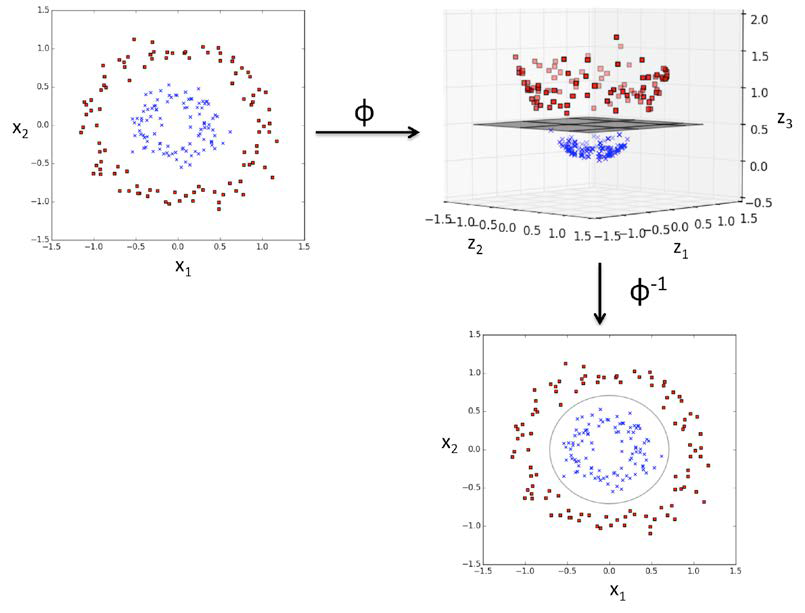
\includegraphics{./pic/chapter-4-3_pic_3.png}
\caption{image.png}
\end{figure}

    \hypertarget{kernel-trick}{%
\subsubsection{Kernel Trick}\label{kernel-trick}}

\textbf{TO BE FINISHED}

    Thanks to the dual formulation in (-) we can see that finding the
\(\alpha\)s depends only on the products
\({\mathbf{x}^{(i)}}^T \mathbf{x}^{(j)}\), and it's easy to observe that
also the classification of new data depends on the product
\({\mathbf{x}^{(i)}}^T \mathbf{u}\).

If we use \(\Phi(\mathbf{x})\) to denote a transformation of the sample
points (into higher dimensions) then the above observation show us that
all we need to know for training and for classifying in the higher
dimensional space are

\[\Phi\left({\mathbf{x}^{(i)}}\right)^T \Phi \left(\mathbf{x}^{(j)}\right)\]

and

\[\Phi \left( {\mathbf{x}^{(i)}}\right)^T \Phi \bigl( \mathbf{u} \bigr) \]

for our transformed data.

\ldots{}

    \begin{tcolorbox}[breakable, size=fbox, boxrule=1pt, pad at break*=1mm,colback=cellbackground, colframe=cellborder]
\prompt{In}{incolor}{13}{\boxspacing}
\begin{Verbatim}[commandchars=\\\{\}]
\PY{k+kn}{from} \PY{n+nn}{matplotlib}\PY{n+nn}{.}\PY{n+nn}{colors} \PY{k+kn}{import} \PY{n}{ListedColormap}

\PY{k}{def} \PY{n+nf}{plot\PYZus{}decision\PYZus{}regions}\PY{p}{(}\PY{n}{X}\PY{p}{,} \PY{n}{y}\PY{p}{,} \PY{n}{classifier}\PY{p}{,} \PY{n}{test\PYZus{}idx}\PY{o}{=}\PY{k+kc}{None}\PY{p}{,} \PY{n}{resolution}\PY{o}{=}\PY{l+m+mf}{0.02}\PY{p}{)}\PY{p}{:}
    \PY{c+c1}{\PYZsh{} setup marker generator and color map}
    \PY{n}{markers} \PY{o}{=} \PY{p}{(}\PY{l+s+s1}{\PYZsq{}}\PY{l+s+s1}{s}\PY{l+s+s1}{\PYZsq{}}\PY{p}{,} \PY{l+s+s1}{\PYZsq{}}\PY{l+s+s1}{x}\PY{l+s+s1}{\PYZsq{}}\PY{p}{,} \PY{l+s+s1}{\PYZsq{}}\PY{l+s+s1}{o}\PY{l+s+s1}{\PYZsq{}}\PY{p}{,} \PY{l+s+s1}{\PYZsq{}}\PY{l+s+s1}{\PYZca{}}\PY{l+s+s1}{\PYZsq{}}\PY{p}{,} \PY{l+s+s1}{\PYZsq{}}\PY{l+s+s1}{v}\PY{l+s+s1}{\PYZsq{}}\PY{p}{)}
    \PY{n}{colors} \PY{o}{=} \PY{p}{(}\PY{l+s+s1}{\PYZsq{}}\PY{l+s+s1}{red}\PY{l+s+s1}{\PYZsq{}}\PY{p}{,} \PY{l+s+s1}{\PYZsq{}}\PY{l+s+s1}{blue}\PY{l+s+s1}{\PYZsq{}}\PY{p}{,} \PY{l+s+s1}{\PYZsq{}}\PY{l+s+s1}{lightgreen}\PY{l+s+s1}{\PYZsq{}}\PY{p}{,} \PY{l+s+s1}{\PYZsq{}}\PY{l+s+s1}{gray}\PY{l+s+s1}{\PYZsq{}}\PY{p}{,} \PY{l+s+s1}{\PYZsq{}}\PY{l+s+s1}{cyan}\PY{l+s+s1}{\PYZsq{}}\PY{p}{)}
    \PY{n}{cmap} \PY{o}{=} \PY{n}{ListedColormap}\PY{p}{(}\PY{n}{colors}\PY{p}{[}\PY{p}{:}\PY{n+nb}{len}\PY{p}{(}\PY{n}{np}\PY{o}{.}\PY{n}{unique}\PY{p}{(}\PY{n}{y}\PY{p}{)}\PY{p}{)}\PY{p}{]}\PY{p}{)}
    \PY{c+c1}{\PYZsh{} plot the decision surface}
    \PY{n}{x1\PYZus{}min}\PY{p}{,} \PY{n}{x1\PYZus{}max} \PY{o}{=} \PY{n}{X}\PY{p}{[}\PY{p}{:}\PY{p}{,} \PY{l+m+mi}{0}\PY{p}{]}\PY{o}{.}\PY{n}{min}\PY{p}{(}\PY{p}{)} \PY{o}{\PYZhy{}} \PY{l+m+mi}{1}\PY{p}{,} \PY{n}{X}\PY{p}{[}\PY{p}{:}\PY{p}{,} \PY{l+m+mi}{0}\PY{p}{]}\PY{o}{.}\PY{n}{max}\PY{p}{(}\PY{p}{)} \PY{o}{+} \PY{l+m+mi}{1}
    \PY{n}{x2\PYZus{}min}\PY{p}{,} \PY{n}{x2\PYZus{}max} \PY{o}{=} \PY{n}{X}\PY{p}{[}\PY{p}{:}\PY{p}{,} \PY{l+m+mi}{1}\PY{p}{]}\PY{o}{.}\PY{n}{min}\PY{p}{(}\PY{p}{)} \PY{o}{\PYZhy{}} \PY{l+m+mi}{1}\PY{p}{,} \PY{n}{X}\PY{p}{[}\PY{p}{:}\PY{p}{,} \PY{l+m+mi}{1}\PY{p}{]}\PY{o}{.}\PY{n}{max}\PY{p}{(}\PY{p}{)} \PY{o}{+} \PY{l+m+mi}{1}
    \PY{n}{xx1}\PY{p}{,} \PY{n}{xx2} \PY{o}{=} \PY{n}{np}\PY{o}{.}\PY{n}{meshgrid}\PY{p}{(}\PY{n}{np}\PY{o}{.}\PY{n}{arange}\PY{p}{(}\PY{n}{x1\PYZus{}min}\PY{p}{,} \PY{n}{x1\PYZus{}max}\PY{p}{,} \PY{n}{resolution}\PY{p}{)}\PY{p}{,}\PY{n}{np}\PY{o}{.}\PY{n}{arange}\PY{p}{(}\PY{n}{x2\PYZus{}min}\PY{p}{,} \PY{n}{x2\PYZus{}max}\PY{p}{,} \PY{n}{resolution}\PY{p}{)}\PY{p}{)}
    \PY{n}{Z} \PY{o}{=} \PY{n}{classifier}\PY{o}{.}\PY{n}{predict}\PY{p}{(}\PY{n}{np}\PY{o}{.}\PY{n}{array}\PY{p}{(}\PY{p}{[}\PY{n}{xx1}\PY{o}{.}\PY{n}{ravel}\PY{p}{(}\PY{p}{)}\PY{p}{,} \PY{n}{xx2}\PY{o}{.}\PY{n}{ravel}\PY{p}{(}\PY{p}{)}\PY{p}{]}\PY{p}{)}\PY{o}{.}\PY{n}{T}\PY{p}{)}
    \PY{n}{Z} \PY{o}{=} \PY{n}{Z}\PY{o}{.}\PY{n}{reshape}\PY{p}{(}\PY{n}{xx1}\PY{o}{.}\PY{n}{shape}\PY{p}{)}
    \PY{n}{plt}\PY{o}{.}\PY{n}{contourf}\PY{p}{(}\PY{n}{xx1}\PY{p}{,} \PY{n}{xx2}\PY{p}{,} \PY{n}{Z}\PY{p}{,} \PY{n}{alpha}\PY{o}{=}\PY{l+m+mf}{0.3}\PY{p}{,} \PY{n}{cmap}\PY{o}{=}\PY{n}{cmap}\PY{p}{)}
    \PY{n}{plt}\PY{o}{.}\PY{n}{xlim}\PY{p}{(}\PY{n}{xx1}\PY{o}{.}\PY{n}{min}\PY{p}{(}\PY{p}{)}\PY{p}{,} \PY{n}{xx1}\PY{o}{.}\PY{n}{max}\PY{p}{(}\PY{p}{)}\PY{p}{)}
    \PY{n}{plt}\PY{o}{.}\PY{n}{ylim}\PY{p}{(}\PY{n}{xx2}\PY{o}{.}\PY{n}{min}\PY{p}{(}\PY{p}{)}\PY{p}{,} \PY{n}{xx2}\PY{o}{.}\PY{n}{max}\PY{p}{(}\PY{p}{)}\PY{p}{)}
    \PY{k}{for} \PY{n}{idx}\PY{p}{,} \PY{n}{cl} \PY{o+ow}{in} \PY{n+nb}{enumerate}\PY{p}{(}\PY{n}{np}\PY{o}{.}\PY{n}{unique}\PY{p}{(}\PY{n}{y}\PY{p}{)}\PY{p}{)}\PY{p}{:}
        \PY{n}{plt}\PY{o}{.}\PY{n}{scatter}\PY{p}{(}\PY{n}{x}\PY{o}{=}\PY{n}{X}\PY{p}{[}\PY{n}{y} \PY{o}{==} \PY{n}{cl}\PY{p}{,} \PY{l+m+mi}{0}\PY{p}{]}\PY{p}{,} 
                    \PY{n}{y}\PY{o}{=}\PY{n}{X}\PY{p}{[}\PY{n}{y} \PY{o}{==} \PY{n}{cl}\PY{p}{,} \PY{l+m+mi}{1}\PY{p}{]}\PY{p}{,}
                    \PY{n}{alpha}\PY{o}{=}\PY{l+m+mf}{0.8}\PY{p}{,} 
                    \PY{n}{c}\PY{o}{=}\PY{n}{colors}\PY{p}{[}\PY{n}{idx}\PY{p}{]}\PY{p}{,}
                    \PY{n}{marker}\PY{o}{=}\PY{n}{markers}\PY{p}{[}\PY{n}{idx}\PY{p}{]}\PY{p}{,} 
                    \PY{n}{label}\PY{o}{=}\PY{n}{cl}\PY{p}{,} 
                    \PY{n}{edgecolor}\PY{o}{=}\PY{l+s+s1}{\PYZsq{}}\PY{l+s+s1}{black}\PY{l+s+s1}{\PYZsq{}}\PY{p}{)}
        
   \PY{c+c1}{\PYZsh{} highlight test examples}
    \PY{k}{if} \PY{n}{test\PYZus{}idx}\PY{p}{:}
        \PY{c+c1}{\PYZsh{} plot all examples}
        \PY{n}{X\PYZus{}test}\PY{p}{,} \PY{n}{y\PYZus{}test} \PY{o}{=} \PY{n}{X}\PY{p}{[}\PY{n}{test\PYZus{}idx}\PY{p}{,} \PY{p}{:}\PY{p}{]}\PY{p}{,} \PY{n}{y}\PY{p}{[}\PY{n}{test\PYZus{}idx}\PY{p}{]}
        \PY{n}{plt}\PY{o}{.}\PY{n}{scatter}\PY{p}{(}\PY{n}{X\PYZus{}test}\PY{p}{[}\PY{p}{:}\PY{p}{,} \PY{l+m+mi}{0}\PY{p}{]}\PY{p}{,} 
                    \PY{n}{X\PYZus{}test}\PY{p}{[}\PY{p}{:}\PY{p}{,} \PY{l+m+mi}{1}\PY{p}{]}\PY{p}{,}
                    \PY{n}{c}\PY{o}{=}\PY{l+s+s1}{\PYZsq{}}\PY{l+s+s1}{\PYZsq{}}\PY{p}{,} 
                    \PY{n}{edgecolor}\PY{o}{=}\PY{l+s+s1}{\PYZsq{}}\PY{l+s+s1}{black}\PY{l+s+s1}{\PYZsq{}}\PY{p}{,} 
                    \PY{n}{alpha}\PY{o}{=}\PY{l+m+mf}{1.0}\PY{p}{,}
                    \PY{n}{linewidth}\PY{o}{=}\PY{l+m+mi}{1}\PY{p}{,} 
                    \PY{n}{marker}\PY{o}{=}\PY{l+s+s1}{\PYZsq{}}\PY{l+s+s1}{o}\PY{l+s+s1}{\PYZsq{}}\PY{p}{,}
                    \PY{n}{s}\PY{o}{=}\PY{l+m+mi}{100}\PY{p}{,} 
                    \PY{n}{label}\PY{o}{=}\PY{l+s+s1}{\PYZsq{}}\PY{l+s+s1}{test set}\PY{l+s+s1}{\PYZsq{}}\PY{p}{)}     
\end{Verbatim}
\end{tcolorbox}

    \begin{tcolorbox}[breakable, size=fbox, boxrule=1pt, pad at break*=1mm,colback=cellbackground, colframe=cellborder]
\prompt{In}{incolor}{14}{\boxspacing}
\begin{Verbatim}[commandchars=\\\{\}]
\PY{k+kn}{from} \PY{n+nn}{sklearn}\PY{n+nn}{.}\PY{n+nn}{svm} \PY{k+kn}{import} \PY{n}{SVC}

\PY{n}{svm} \PY{o}{=} \PY{n}{SVC}\PY{p}{(}\PY{n}{kernel}\PY{o}{=}\PY{l+s+s1}{\PYZsq{}}\PY{l+s+s1}{rbf}\PY{l+s+s1}{\PYZsq{}}\PY{p}{,} \PY{n}{random\PYZus{}state}\PY{o}{=}\PY{l+m+mi}{1}\PY{p}{,} \PY{n}{gamma}\PY{o}{=}\PY{l+m+mf}{0.10}\PY{p}{,} \PY{n}{C}\PY{o}{=}\PY{l+m+mf}{10.0}\PY{p}{)}
\PY{n}{svm}\PY{o}{.}\PY{n}{fit}\PY{p}{(}\PY{n}{X\PYZus{}xor}\PY{p}{,} \PY{n}{y\PYZus{}xor}\PY{p}{)}
\PY{n}{plot\PYZus{}decision\PYZus{}regions}\PY{p}{(}\PY{n}{X\PYZus{}xor}\PY{p}{,} \PY{n}{y\PYZus{}xor}\PY{p}{,} \PY{n}{classifier}\PY{o}{=}\PY{n}{svm}\PY{p}{)}
\PY{n}{plt}\PY{o}{.}\PY{n}{legend}\PY{p}{(}\PY{n}{loc}\PY{o}{=}\PY{l+s+s1}{\PYZsq{}}\PY{l+s+s1}{upper left}\PY{l+s+s1}{\PYZsq{}}\PY{p}{)}
\PY{n}{plt}\PY{o}{.}\PY{n}{tight\PYZus{}layout}\PY{p}{(}\PY{p}{)}
\PY{n}{plt}\PY{o}{.}\PY{n}{show}\PY{p}{(}\PY{p}{)}
\end{Verbatim}
\end{tcolorbox}

    \begin{center}
    \adjustimage{max size={0.9\linewidth}{0.9\paperheight}}{output_47_0.png}
    \end{center}
    { \hspace*{\fill} \\}
    
    \hypertarget{predicting-a-continuous-variable}{%
\subsection{Predicting a Continuous
Variable}\label{predicting-a-continuous-variable}}

    \textbf{TO BE DONE}

    \begin{tcolorbox}[breakable, size=fbox, boxrule=1pt, pad at break*=1mm,colback=cellbackground, colframe=cellborder]
\prompt{In}{incolor}{ }{\boxspacing}
\begin{Verbatim}[commandchars=\\\{\}]

\end{Verbatim}
\end{tcolorbox}


    % Add a bibliography block to the postdoc
    
    
    
\end{document}
